%!TEX root = /Users/mpking/Dropbox/writing/king_dissertation/king_dissertation_master.tex

\chapter{Experimental Investigation of Electron-Induced SEUs} % (fold)
\label{cha:experimental_investigation_of_electron_induced_seus}
This chapter presents experimental methods for \emph{in situ} X-ray irradiation and SEU measurements as a technique for investigating electron-induced SEUs in SRAMs. 
Extensive parametric and functionality testing of SRAM test chips fabricated in 28~nm and 45~nm bulk silicon technology was performed to determine the range of operational stability.
SRAM test chips were shown to be stable and hold valid data over a wide range of supply voltage conditions.
Test boards were designed and integrated to allow independent, simultaneous control of the SRAM test chips and power supply conditions during the experiment.
Test chips were exposed to a source of energetic X-rays from an ARACOR 4100 X-ray irradiator.
SRAMs were programmed into either an all zero (\emph{0000}), all one (\emph{1111}), checkerboard (\emph{1010}), or reverse checkerboard (\emph{0101}) pattern during irradiation.
Once exposure of the SRAM test chip to X-rays was complete, the final state of the data pattern was read back and compared to the initial, programmed, state.
The data pattern and address location of any errors was logged and recorded for further analysis.
Section~\ref{sec:experimental_setup_and_methods} discusses the relevant experimental setup and methods.
Section~\ref{sec:experimental_results} provides a full discussion of the experimental results and analyzes critical experimental parameters.
Section~\ref{sec:comparison_to_low_energy_proton_and_muon_seus} compares the supply voltage dependence of electron-induced SEUs to similar data obtained in muon and low-energy proton irradiations.
 
\section{Experimental Setup and Methods} % (fold)
\label{sec:experimental_setup_and_methods}
A diagram of the experimental setup used to investigate electron-induced SEUs is shown in Fig.~\ref{fig:exp_diagram}. 
An automated test system was developed to allow independent control of two Keithley 2410 SourceMeters\textregistered~for the SRAM test chip and SRAM test board through a GPIB/LAN gateway while sending control commands to the SRAM test board through a USB connection. 
This configuration allows remote control of the SRAM supply voltage and allows the power supply current to be monitored while performing parametric testing of the SRAM test chip.
\begin{figure}[tb]
    \centering
        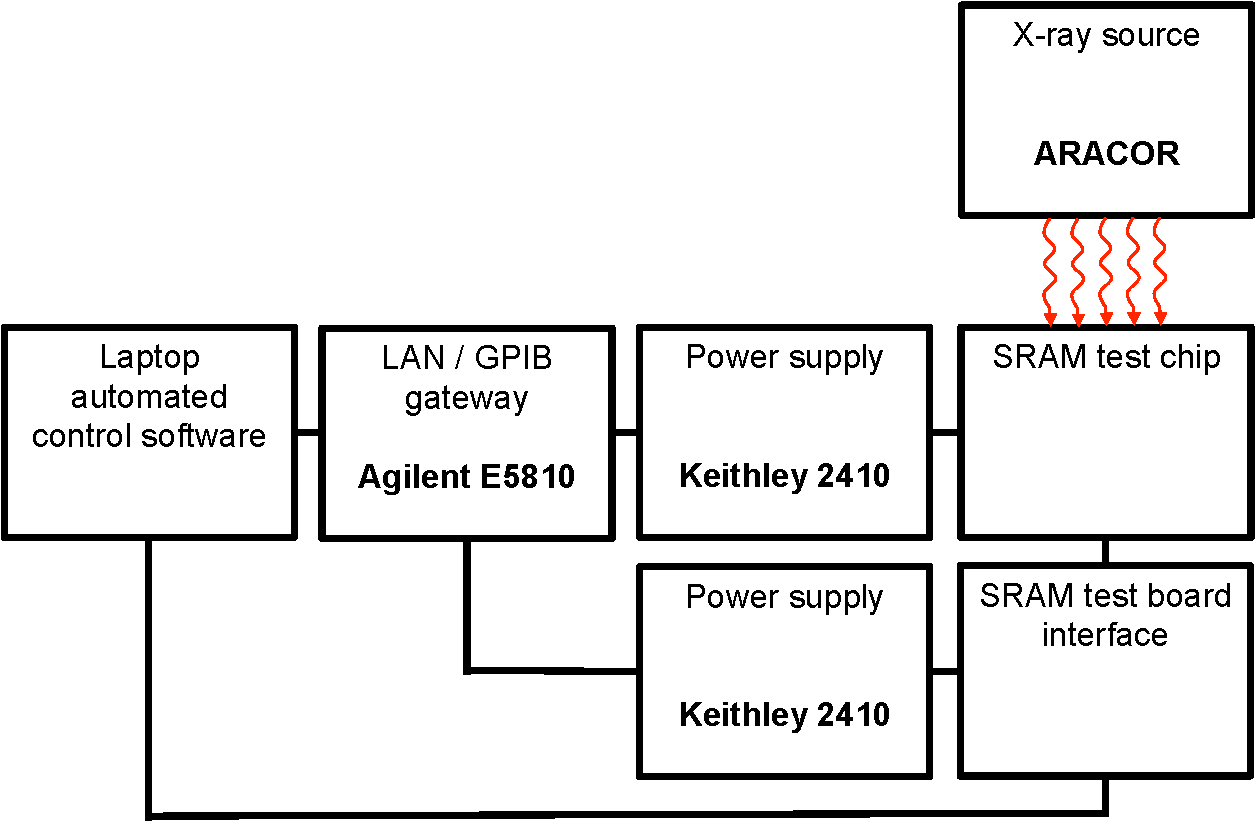
\includegraphics[width=4.5in]{exp_setup.pdf}
        \caption{An automated test system allows independent control of two Keithley 2410 SourceMeters® for the SRAM test chip and test board interface through a LAN/GPIB gateway. Control commands are transmitted to the SRAM test board through a USB connection from a laptop. This system allows the supply voltage of the SRAM to be modulated \emph{in situ}. The device under test is exposed to energetic X-rays under varied supply voltage conditions.}
        \label{fig:exp_diagram}
\end{figure}

Reduced supply voltage conditions are employed to determine the susceptibility of the SRAM to singly-charged particles and compare the bias dependence of electron-induced upset rates to that of upsets known to be caused by low-energy protons and muons \cite{Rodbell:2007vl, Sierawski:2010cj}.
As discussed in Section~\ref{sec:basic_sram_topology_and_operation}, low-voltage operation has practical significance, since it is common for SRAMs in standby mode to operate at 70-80\% of the nominal supply voltage to reduce power consumption \cite{semeraro:2002dvfs,david:2011dvfs}.
Low-power applications, mobile communications, mobile computing, and medical devices also frequently employ power-saving techniques that include reducing $V_{DD}$ during standby and idle modes of operation, making this a relevant testing approach.

Fig.~\ref{fig:exp_timing_diagram} shows the applied bias as a function of time for a representative testing sequence employed in this study. 
An initial write and read, using either an all one, all zero, checkerboard or reverse checkerboard pattern, is performed at nominal bias conditions prior to X-ray exposure of the device under test (DUT). 
The supply voltage is then lowered while the DUT is irradiated. In the case of Fig.~\ref{fig:exp_timing_diagram}, the total exposure time was 30 seconds. 
In other experiments the total exposure time was varied from 30 seconds to several minutes. 
Once the X-ray source was turned off, the supply voltage was returned to nominal conditions and the final state of the memory was read. 
The final and initial states of the memory were compared to identify any errors that may have occurred, noting the address and data patterns of observed errors for post-processing.

\begin{figure}[tb]
    \centering
        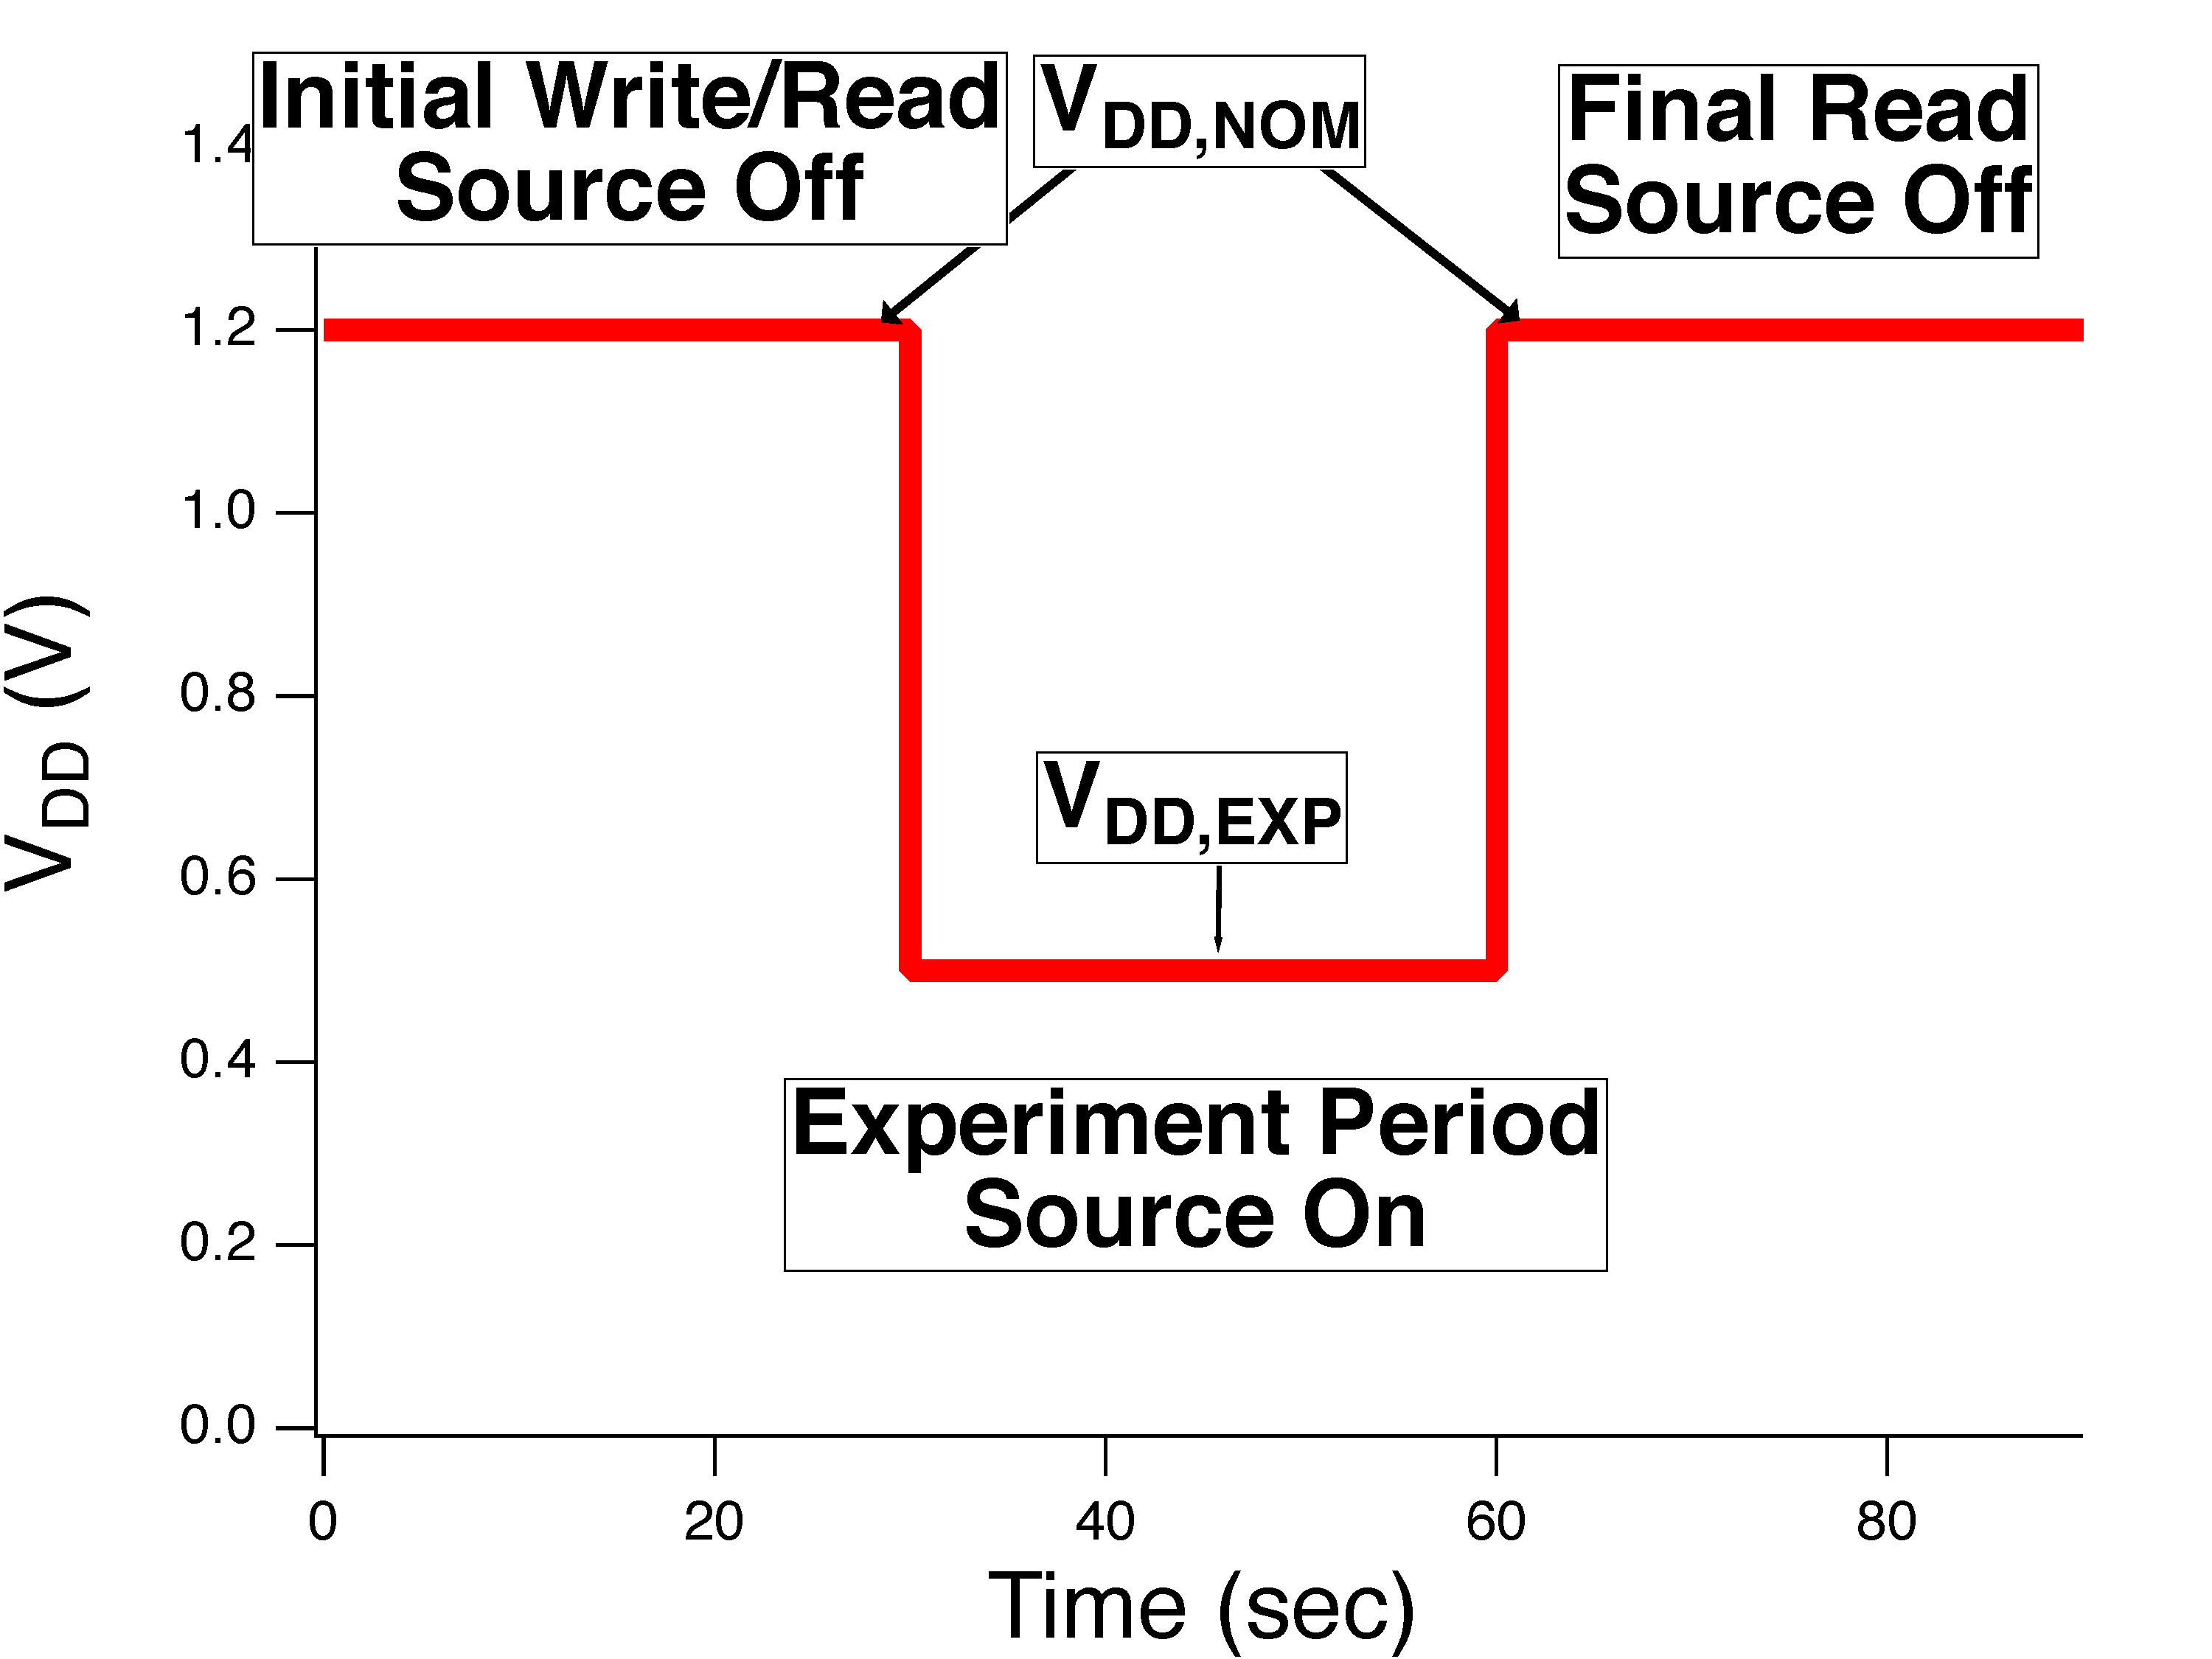
\includegraphics[width=4.5in]{timing_diagram_ppt.pdf}
        \caption{Example timing diagram for measuring upsets at reduced bias. Read and write operations are performed under nominal bias condition, V$_{DDNOM}$. During exposure the rail is reduced to a value, V$_{DDEXP}$, for the duration of the experiment. Upon conclusion of the exposure, the nominal rail is restored, a final read operation is performed, and any errors recorded.}
        \label{fig:exp_timing_diagram}
\end{figure}

During the experimental period the range of supply voltages used in this study varies from 0.35-1.0~V. 
The SRAM test chips used in this work are commercial parts \emph{designed} to operate and remain stable between 0.5-1.0~V.
In functionality and parametric bench testing, the test chips were confirmed to be stable down to 0.35~V during a one hour testing period, which is much longer than typical X-ray exposure times.
Extensive testing was done prior to irradiation to demonstrate that no bit flips occurred under any bias conditions, indicating the memory was written properly and held valid information through the timing sequence shown in Fig.~\ref{fig:exp_timing_diagram} and in all other cases shown in this work. 
Functionality and parametric testing was performed before and after each radiation exposure for equivalent time periods to ensure the integrity of the SRAM under all bias conditions. 
This procedure verifies that the data remain intact and stable at all supply voltage conditions and that no degradation due to TID has occurred during or after each X-ray exposure.

\begin{figure}[tb]
    \centering
        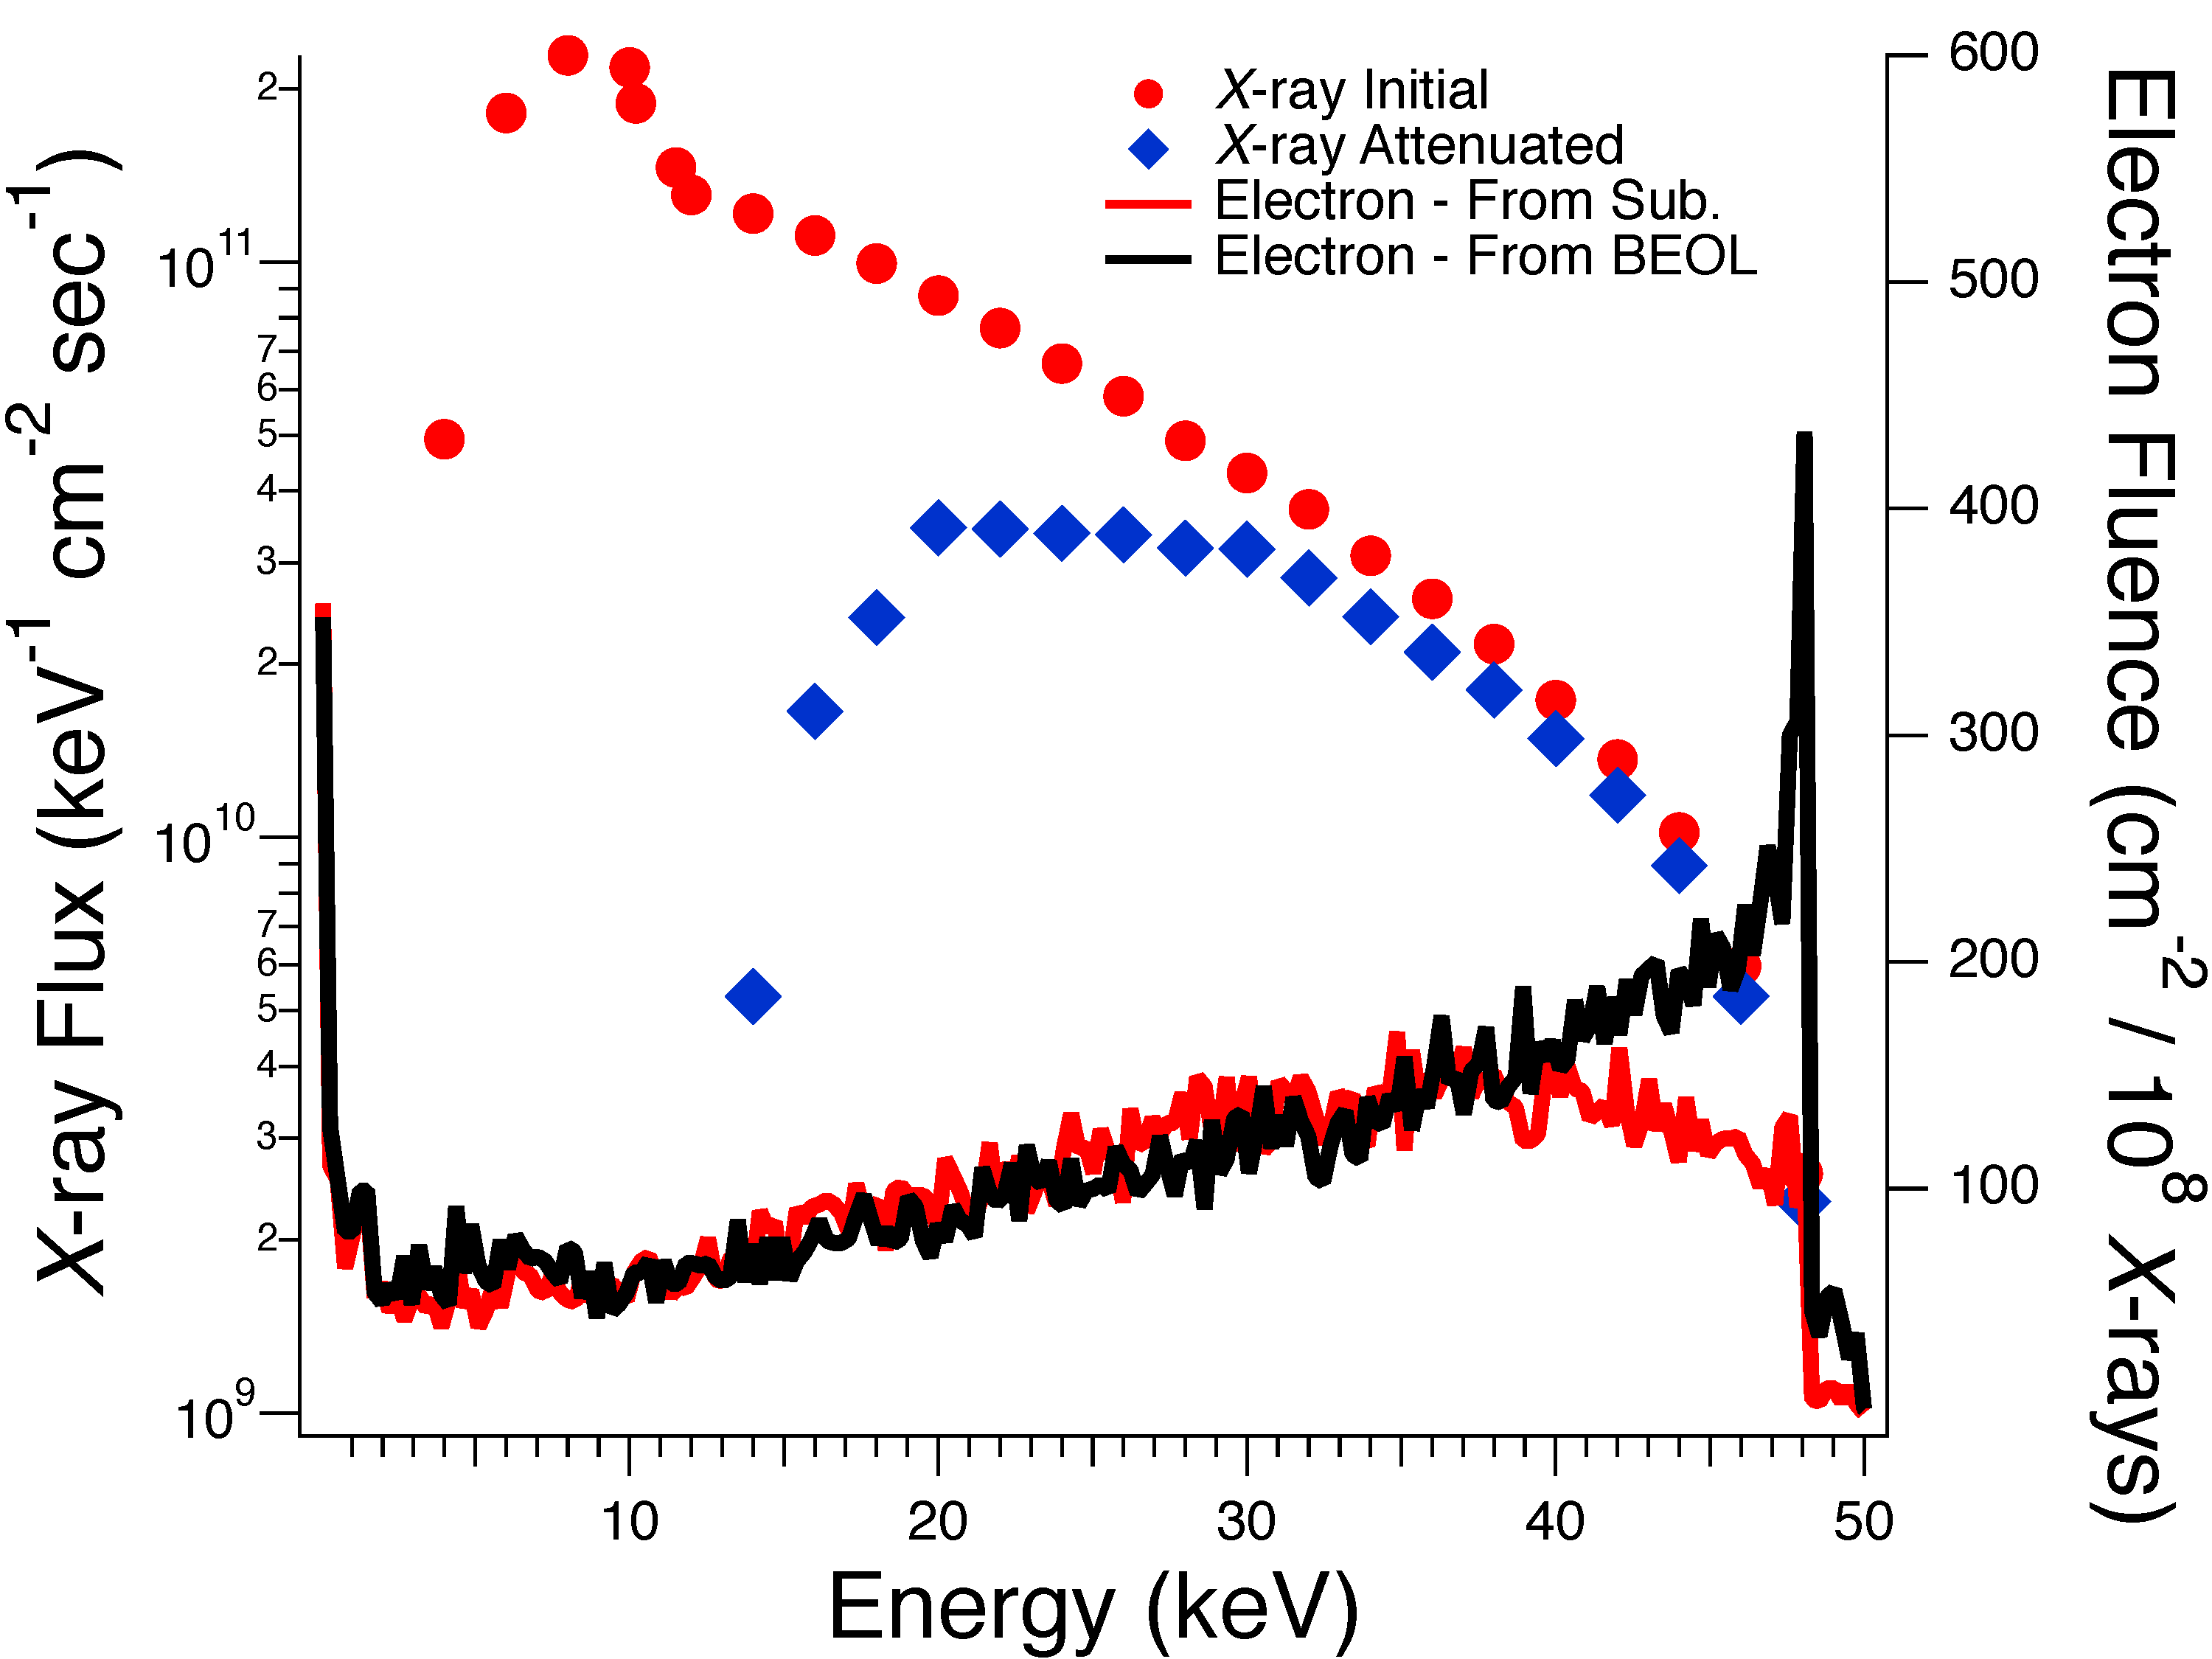
\includegraphics[width=5in]{aracor_spectrum_elec_fluence.pdf}
        \caption
        [X-ray and electron spectra produced by the ARACOR 4100 X-ray irradiator. The average energy is 10~keV and the maximum energy is 50~keV, corresponding to the endpoint bremsstrahlung energy. For the error rate testing in this study, the spectrum is modified by a 1~mm aluminum attenuator, which reduces the flux of low-energy X-rays incident onto the DUT. The electron fluences corresponding to monoenergetic 50~keV X-rays interacting with the active silicon region in the ``forward'' (scattering events in the active device overlayer materials, denoted BEOL) and ``reverse'' (scattering events in the device substrate) beam directions are shown on the right.]
        {X-ray and electron spectra produced by the ARACOR 4100 X-ray irradiator. The average energy is 10~keV and the maximum energy is 50~keV, corresponding to the endpoint bremsstrahlung energy \cite{Dozier:1983wx, Fleetwood:1986ug}. For the error rate testing in this study, the spectrum is modified by a 1~mm aluminum attenuator, which reduces the flux of low-energy X-rays incident onto the DUT. The electron fluences corresponding to monoenergetic 50~keV X-rays interacting with the active silicon region in the ``forward'' (scattering events in the active device overlayer materials, denoted BEOL) and ``reverse'' (scattering events in the device substrate) beam directions are shown on the right.}
        \label{fig:aracor_spectrum}
\end{figure}
Irradiation was performed with a beam current of 1~mA and beam voltage of 50~kV. 
The X-ray spectra produced under these conditions are shown in Fig.~\ref{fig:aracor_spectrum} \cite{Dozier:1983wx, Fleetwood:1986ug}. 
For the unattenuated spectrum in Fig.~\ref{fig:aracor_spectrum}, 10~keV is the average energy and 50~keV is the endpoint bremsstrahlung energy. 
The interaction between X-rays in this energy range and electrons is dominated by the photoelectric effect, however, near the bremsstrahlung edge Compton scattering becomes a non-negligible contribution. 
The generated photo-electrons in these interactions are emitted omnidirectionally.
As discussed in Section~\ref{sub:photon_transport}, for highly energetic photons, where the energy of the incident photon is much greater than the photo-electron shell binding energy ($\hbar \omega \gg E_b$), most of the absorbed photon energy is transferred to the photo-electron.

A 1 mm aluminum attenuator was placed above the DUT with an air gap of 3.5~cm between the attenuator and the test chip.
The attenuator filters the low-energy X-ray spectrum, passing the more energetic X-rays that are more likely to produce observable electron-induced effects. 
This reduces the dose-rate and TID effects. 
Attenuation of the initial spectrum by the 1 mm layer of aluminum is calculated using the Beer-Lambert law, Eq.~\ref{eq:beer_lambert} and plotted in Fig.~\ref{fig:aracor_spectrum}.
The prominent 10~keV X-ray peak is absent from the attenuated spectrum; only the high energy tail of the X-ray distribution is capable of transporting through the attenuator and interacting with the DUT.
The majority of photo-electrons generated in the attenuator are reabsorbed before leaving the Al.

\begin{figure}[tb]
    \begin{center}
        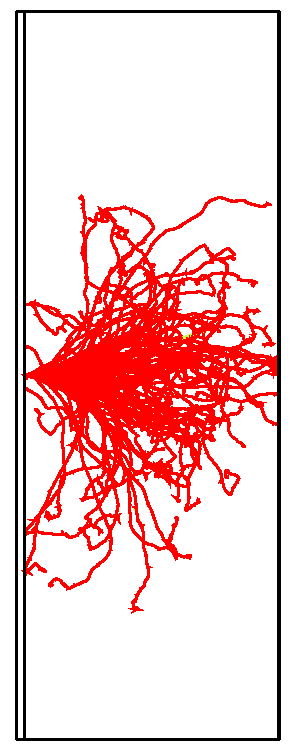
\includegraphics[height=5in, angle=-90]{e-air-50keV-100events_cropped.pdf}
    \end{center}
    \caption{50~keV photo-electrons exiting the aluminum attenuator have insufficient energy to transport through the 3.5~cm air gap and back end of line (BEOL) materials to reach the active silicon. Only photo-electrons generated in the DUT itself can interact with the device material in the sensitive silicon region.}
    \label{fig:air_gap}
\end{figure}

Fig.~\ref{fig:air_gap} shows the transport of maximal energy, 50~keV, photo-electrons generated at the Al-to-air interface. 
The Al is on top and the air gap is the large rectangle.
The DUT is very thin and on the bottom of the figure.
Photo-electrons have random trajectories. 
The few electrons that transport through the air gap to the DUT stop within the first few micrometers of the back end of line (BEOL) materials (metallization and dielectric layers) \cite{Dasgupta:2011mg}.
Therefore, only X-rays absorbed within the DUT itself generate photo-electrons that can interact with the device material in the sensitive volume of the device.
An example of this type of interaction is shown in Fig.~\ref{fig:photoabsorption_opendx} where the absorption of an incident 10~keV X-ray leads to the generation of an initially free, nearly ballistic electron that deposits 9.3~keV of energy when it scatters within the sensitive volume of a 45~nm SRAM.

\begin{figure}[htbp]
    \centering
        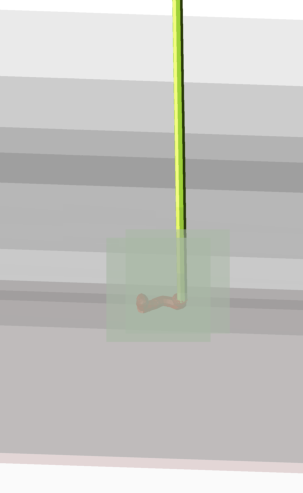
\includegraphics[width=3.75in]{image_1_box_2_flat3d.pdf}
        \caption{A 10~keV X-ray is normally incident on the simulated device structure of a 45~nm SRAM. It subsequently undergoes photoabsorption resulting in the generation of a energetic electron. The resulting electron then transports through the device material, depositing energy in excess of 9.3~keV within the sensitive volume of the SRAM.}
        \label{fig:photoabsorption_opendx}
\end{figure}

The electron fluence spectrum corresponding to a monoenergetic beam of 50~keV X-rays in the ``forward'' and ``reverse'' beam direction is plotted on the right hand side of Fig.~\ref{fig:aracor_spectrum}.
The most frequent energy corresponds to the incident X-ray energy in the forward direction, which corresponds to photo-electrons generated in the BEOL materials and the active silicon region.
In the reverse beam direction, corresponding to electrons generated in the substrate that transport back to the active silicon, the situation is more complicated due to the random trajectory of the generated photo-electrons. 
This demonstrates the random nature, in energy and trajectory, of the electron environment local to the sensitive volume.

Following the method used in \cite{Fleetwood:1986ug}, flatband voltage, $V_{FB}$, shifts were measured with MOS capacitors to calibrate the dose-rate. 
The devices were fabricated and packaged at Sandia National Laboratories; lids were removed for the X-ray irradiations. 
The calibration devices were $n$-type substrate MOS capacitors featuring aluminum dot gates with an area of 0.01~cm$^2$ and SiO$_2$ gate oxide thickness of 101~nm \cite{Schwank:1987fq}. 
\begin{figure}[tb]
    \centering
        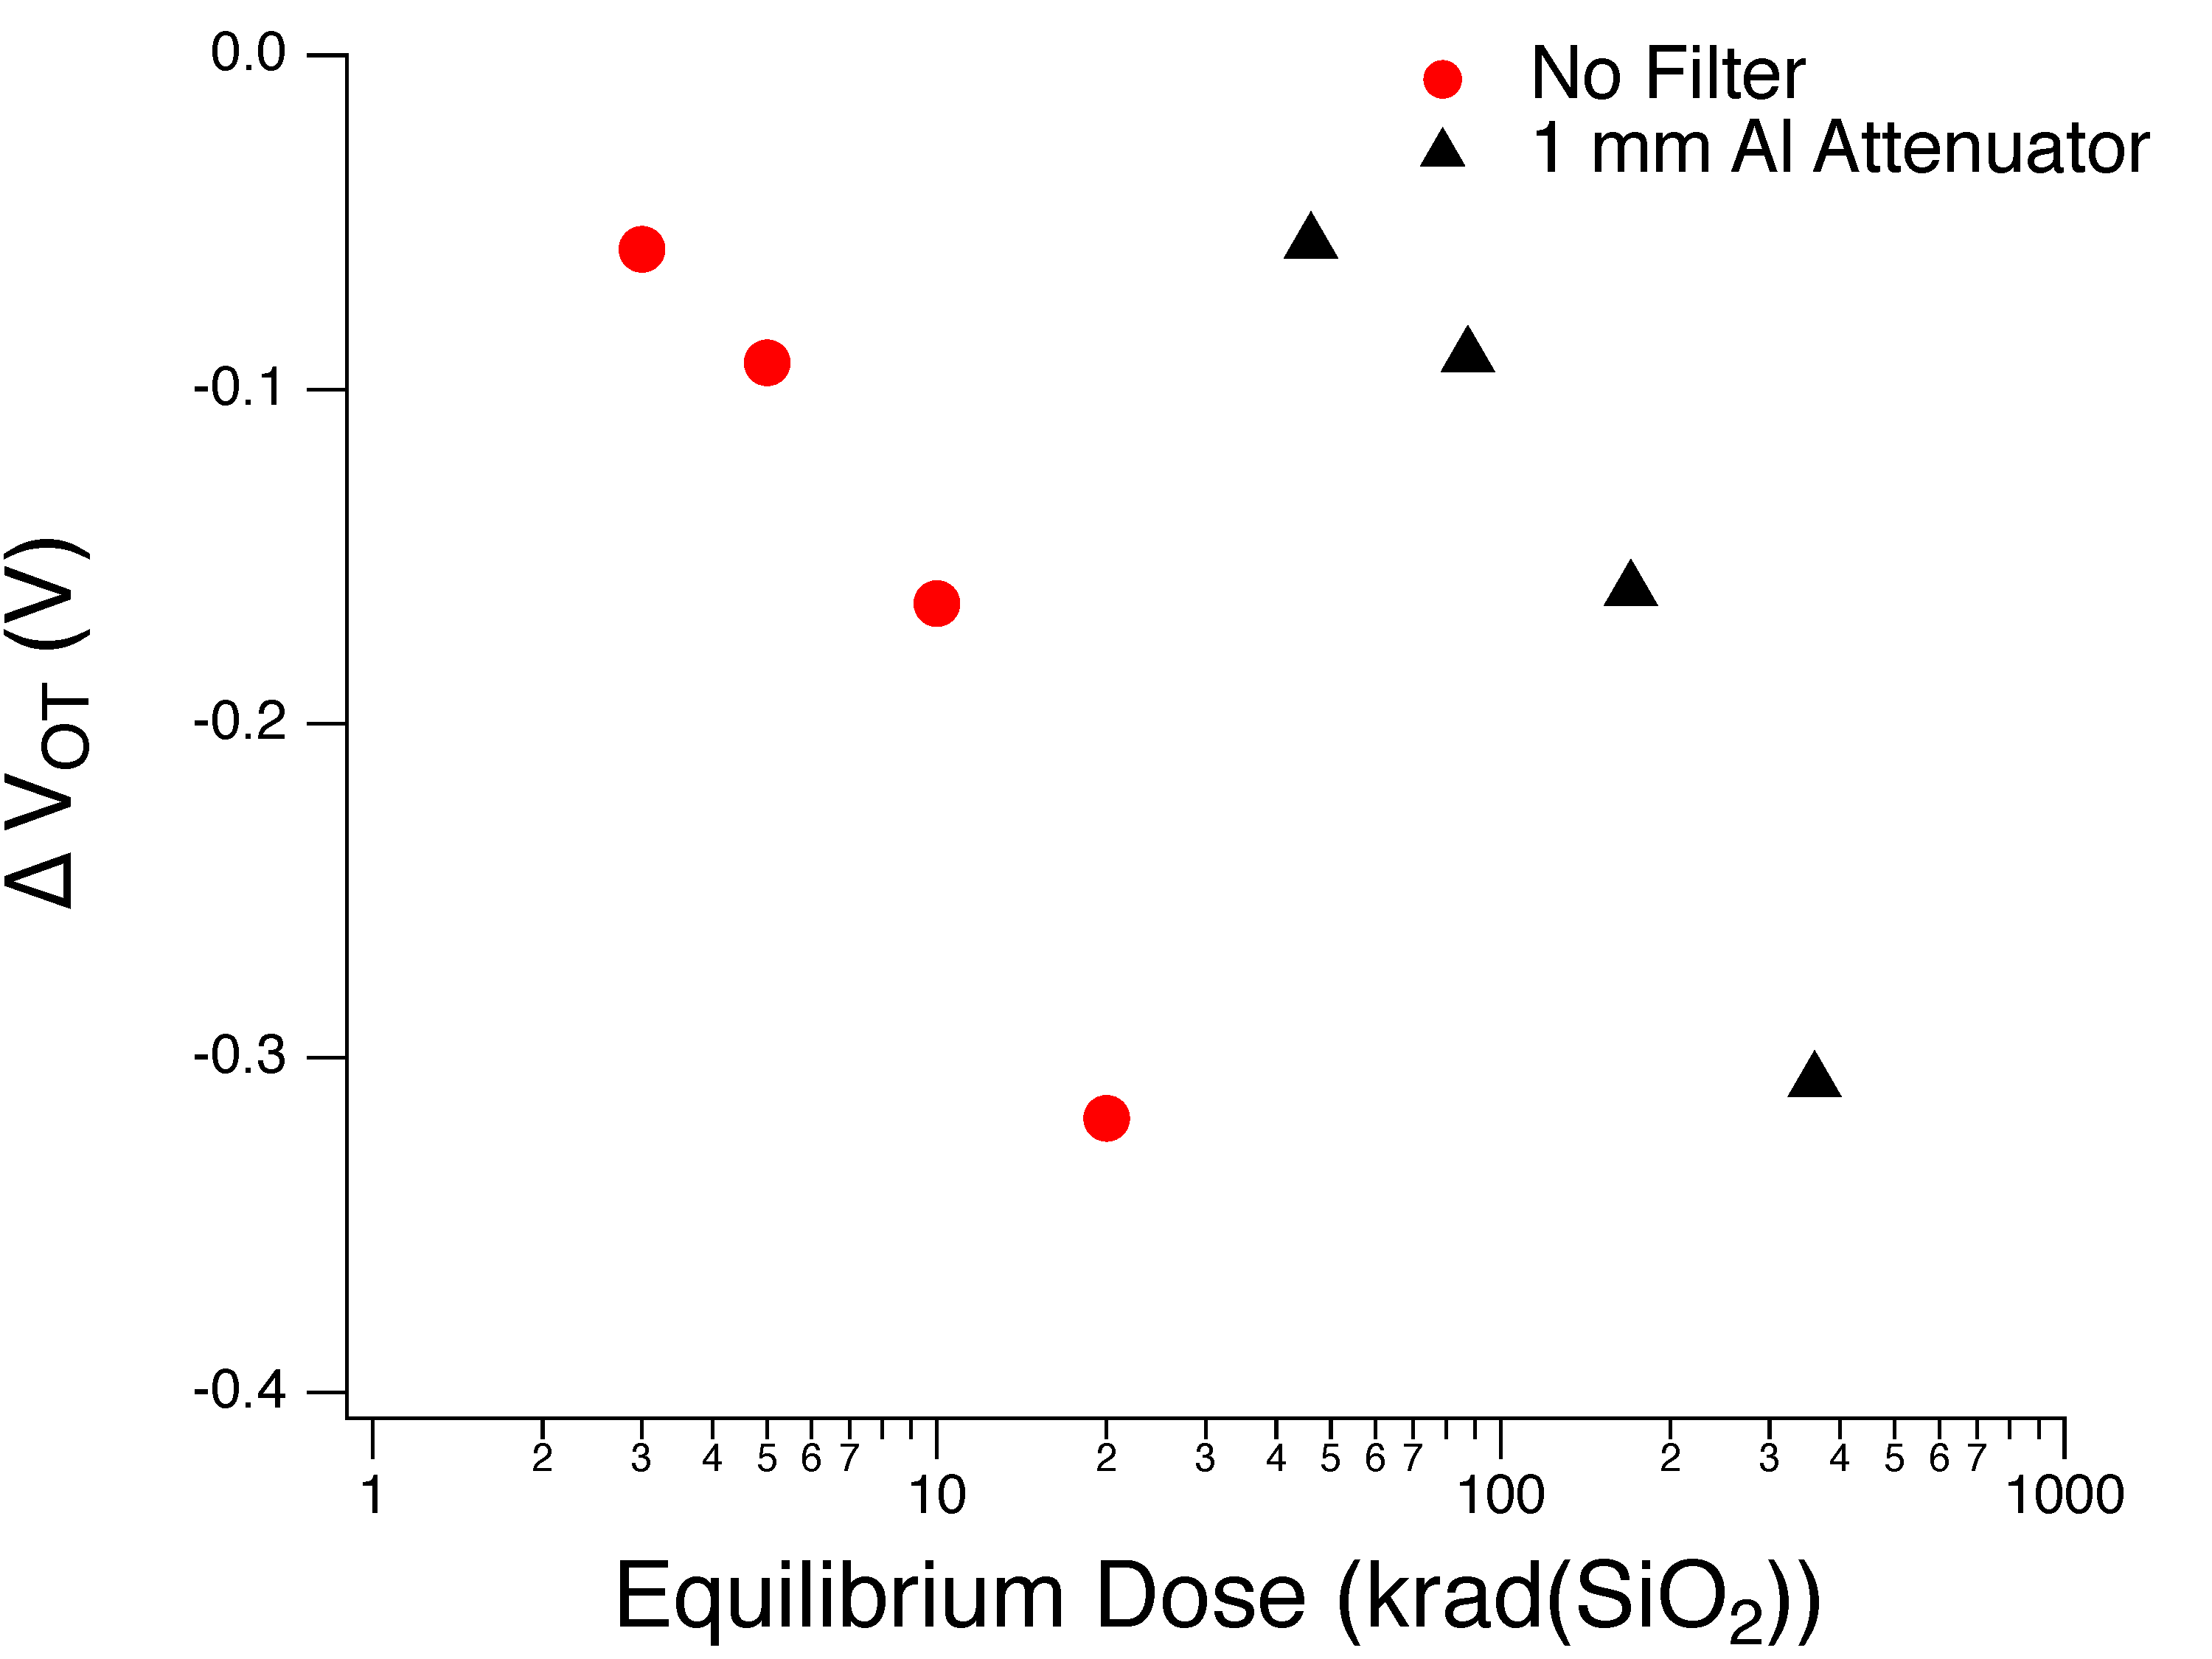
\includegraphics[width=5in]{delta_vot_vs_dose_ppt.pdf}
    \caption{$\Delta V_{OT}$ as a function of equilibrium dose for MOS capacitors irradiated with beam current and voltage of 1~mA and 50~kV, respectively. Devices were biased with 10~V on the gate during irradiation. The use of a 1~mm Al attenuator causes a increase in equilibrium dose required to achieve equivalent shifts in $\Delta V_{OT}$ by a factor of 17, indicating the nominal dose rate of 1.7~krad(SiO$_2$)/min is reduced to 100~rad(SiO$_2$)/min.}
    \label{fig:delta_vot_vs_dose}
\end{figure}
The dose-rate calibration data are plotted in Fig.~\ref{fig:delta_vot_vs_dose}, which shows the change in oxide-trapped charge as determined by shifts in \emph{C-V} characteristics.
The equilibrium dose shown in Fig.~\ref{fig:delta_vot_vs_dose} represents the nominal, unattenuated dose from the X-ray source. 
The measured dose-rate incident on the MOS capacitor is reduced by a factor of 17 when compared to the nominal dose-rate \cite{Fleetwood:1986ug}. 
The attenuated dose-rate is 100~rad(SiO$_2$)/min. 

The X-ray flux is calculated by integrating over the attenuated energy spectrum in Fig.~\ref{fig:aracor_spectrum} and can be calculated as
\begin{equation}
    \label{eq:cum_pho_flux}
    \phi_{total} = \sum_{i=0}^{\infty} \phi(E_{i})
\end{equation}
where $\phi(E_{i})$ is the flux of photons with energy $E_{i}$, and $\phi_{total}$ represents a cumulative photon flux. 
Evaluating Eq.~\ref{eq:cum_pho_flux} with the attenuated photon spectrum yields a cumulative photon flux of 1.5$\times$10$^{12}$~cm$^{-2}$~s$^{-1}$.
Similarly, the electron flux corresponding to 50~keV X-rays is calculated to be 1.16$\times$10$^{6}$~cm$^{-2}$~s$^{-1}$.
% section experimental_setup_and_methods (end)

\section{Experimental Results} % (fold)
\label{sec:experimental_results}
Using the methods described in Section~\ref{sec:experimental_setup_and_methods}, several experiments exposing SRAMs to energetic X-rays were performed to investigate the plausibility of electron-induced upset events. 
Four types of devices were used. 
Test Chips A and B are 28~nm SRAMs with a capacity of 23~Mbit and nominal operating voltage of 0.9~V in triple-well (TW) and dual-well (DW) processes, respectively. 
Test Chip C is a 28~nm SRAM with a capacity of 32~Mbit and nominal operating voltage of 1.0~V. 
Test Chip D is a 45~nm SRAM with a capacity of 4~Mbit and nominal operating voltage of 1.1~V. 
Normalized cross-sections are obtained for each applied bias condition using the following relationship,
\begin{equation}
    \label{eq:norm_cs}
    \sigma(V_{DD}) = \frac{N}{A_{cell} \Phi}
\end{equation}
where $N$ is the number of observed errors, $A_{cell}$ is the cell area of the SRAM being tested, and $\Phi$ is the photon fluence. 
Error bars are shown at the one-sigma confidence interval in all experimental and simulated cross-sections.
Table~\ref{table:exp_times} shows the experimental supply voltage conditions, exposure time, and corresponding X-ray fluence for measurements on each test chip.

\begin{table}[tb]
    \caption{X-ray Supply Voltage, Exposure Time, and Fluence}
    \centering
        \begin{tabular}{c|cc|cc}
        \hline\hline
        & \multicolumn{2}{c |}{Test Chip A} & \multicolumn{2}{c}{Test Chip B} \\ 
        $V_{DD}$ (V) & Time (s) & Fluence (cm$^{-2}$) & Time (s) & Fluence (cm$^{-2}$)\\
        \hline\hline
        0.35 & 40 & 6$\times$10$^{13}$ & 40 & 6$\times$10$^{13}$ \\
        0.4 & 130 & 1.95$\times$10$^{14}$ & 120 & 1.8$\times$10$^{14}$ \\
        0.5 & 310 & 4.65$\times$10$^{14}$ & 300 & 4.5$\times$10$^{14}$ \\
        0.6 & 620 & 9.3$\times$10$^{14}$ & 630 & 9.45$\times$10$^{14}$ \\
        0.7 & & & 1260 & 1.89$\times$10$^{15}$ \\
        0.8 & & & 630 & 9.45$\times$10$^{14}$\\
        \hline\hline
        & \multicolumn{2}{c |}{Test Chip C} & \multicolumn{2}{c}{Test Chip D} \\ 
        $V_{DD}$ (V) & Time (s) & Fluence (cm$^{-2}$) & Time (s) & Fluence (cm$^{-2}$)\\
        \hline\hline
        0.45 & 90 & 1.35$\times$10$^{14}$ & 270 & 4.05$\times$10$^{14}$ \\
        0.5 & 180 & 2.7$\times$10$^{14}$ & 30 & 4.5$\times$10$^{13}$ \\
        0.55 & 180 & 2.7$\times$10$^{14}$ & 360 & 5.4$\times$10$^{14}$ \\
        0.6 & 540 & 8.1$\times$10$^{14}$ & 860 & 1.29$\times$10$^{15}$ \\
        0.65 & 300 & 4.5$\times$10$^{14}$ & 1080 & 1.62$\times$10$^{15}$ \\
        0.7 & 600 & 9$\times$10$^{14}$ & 528 & 7.92$\times$10$^{14}$ \\
        \hline
        \end{tabular}
        \label{table:exp_times}
    %\end{centering}
\end{table}

\begin{figure}[tb]
    \centering
        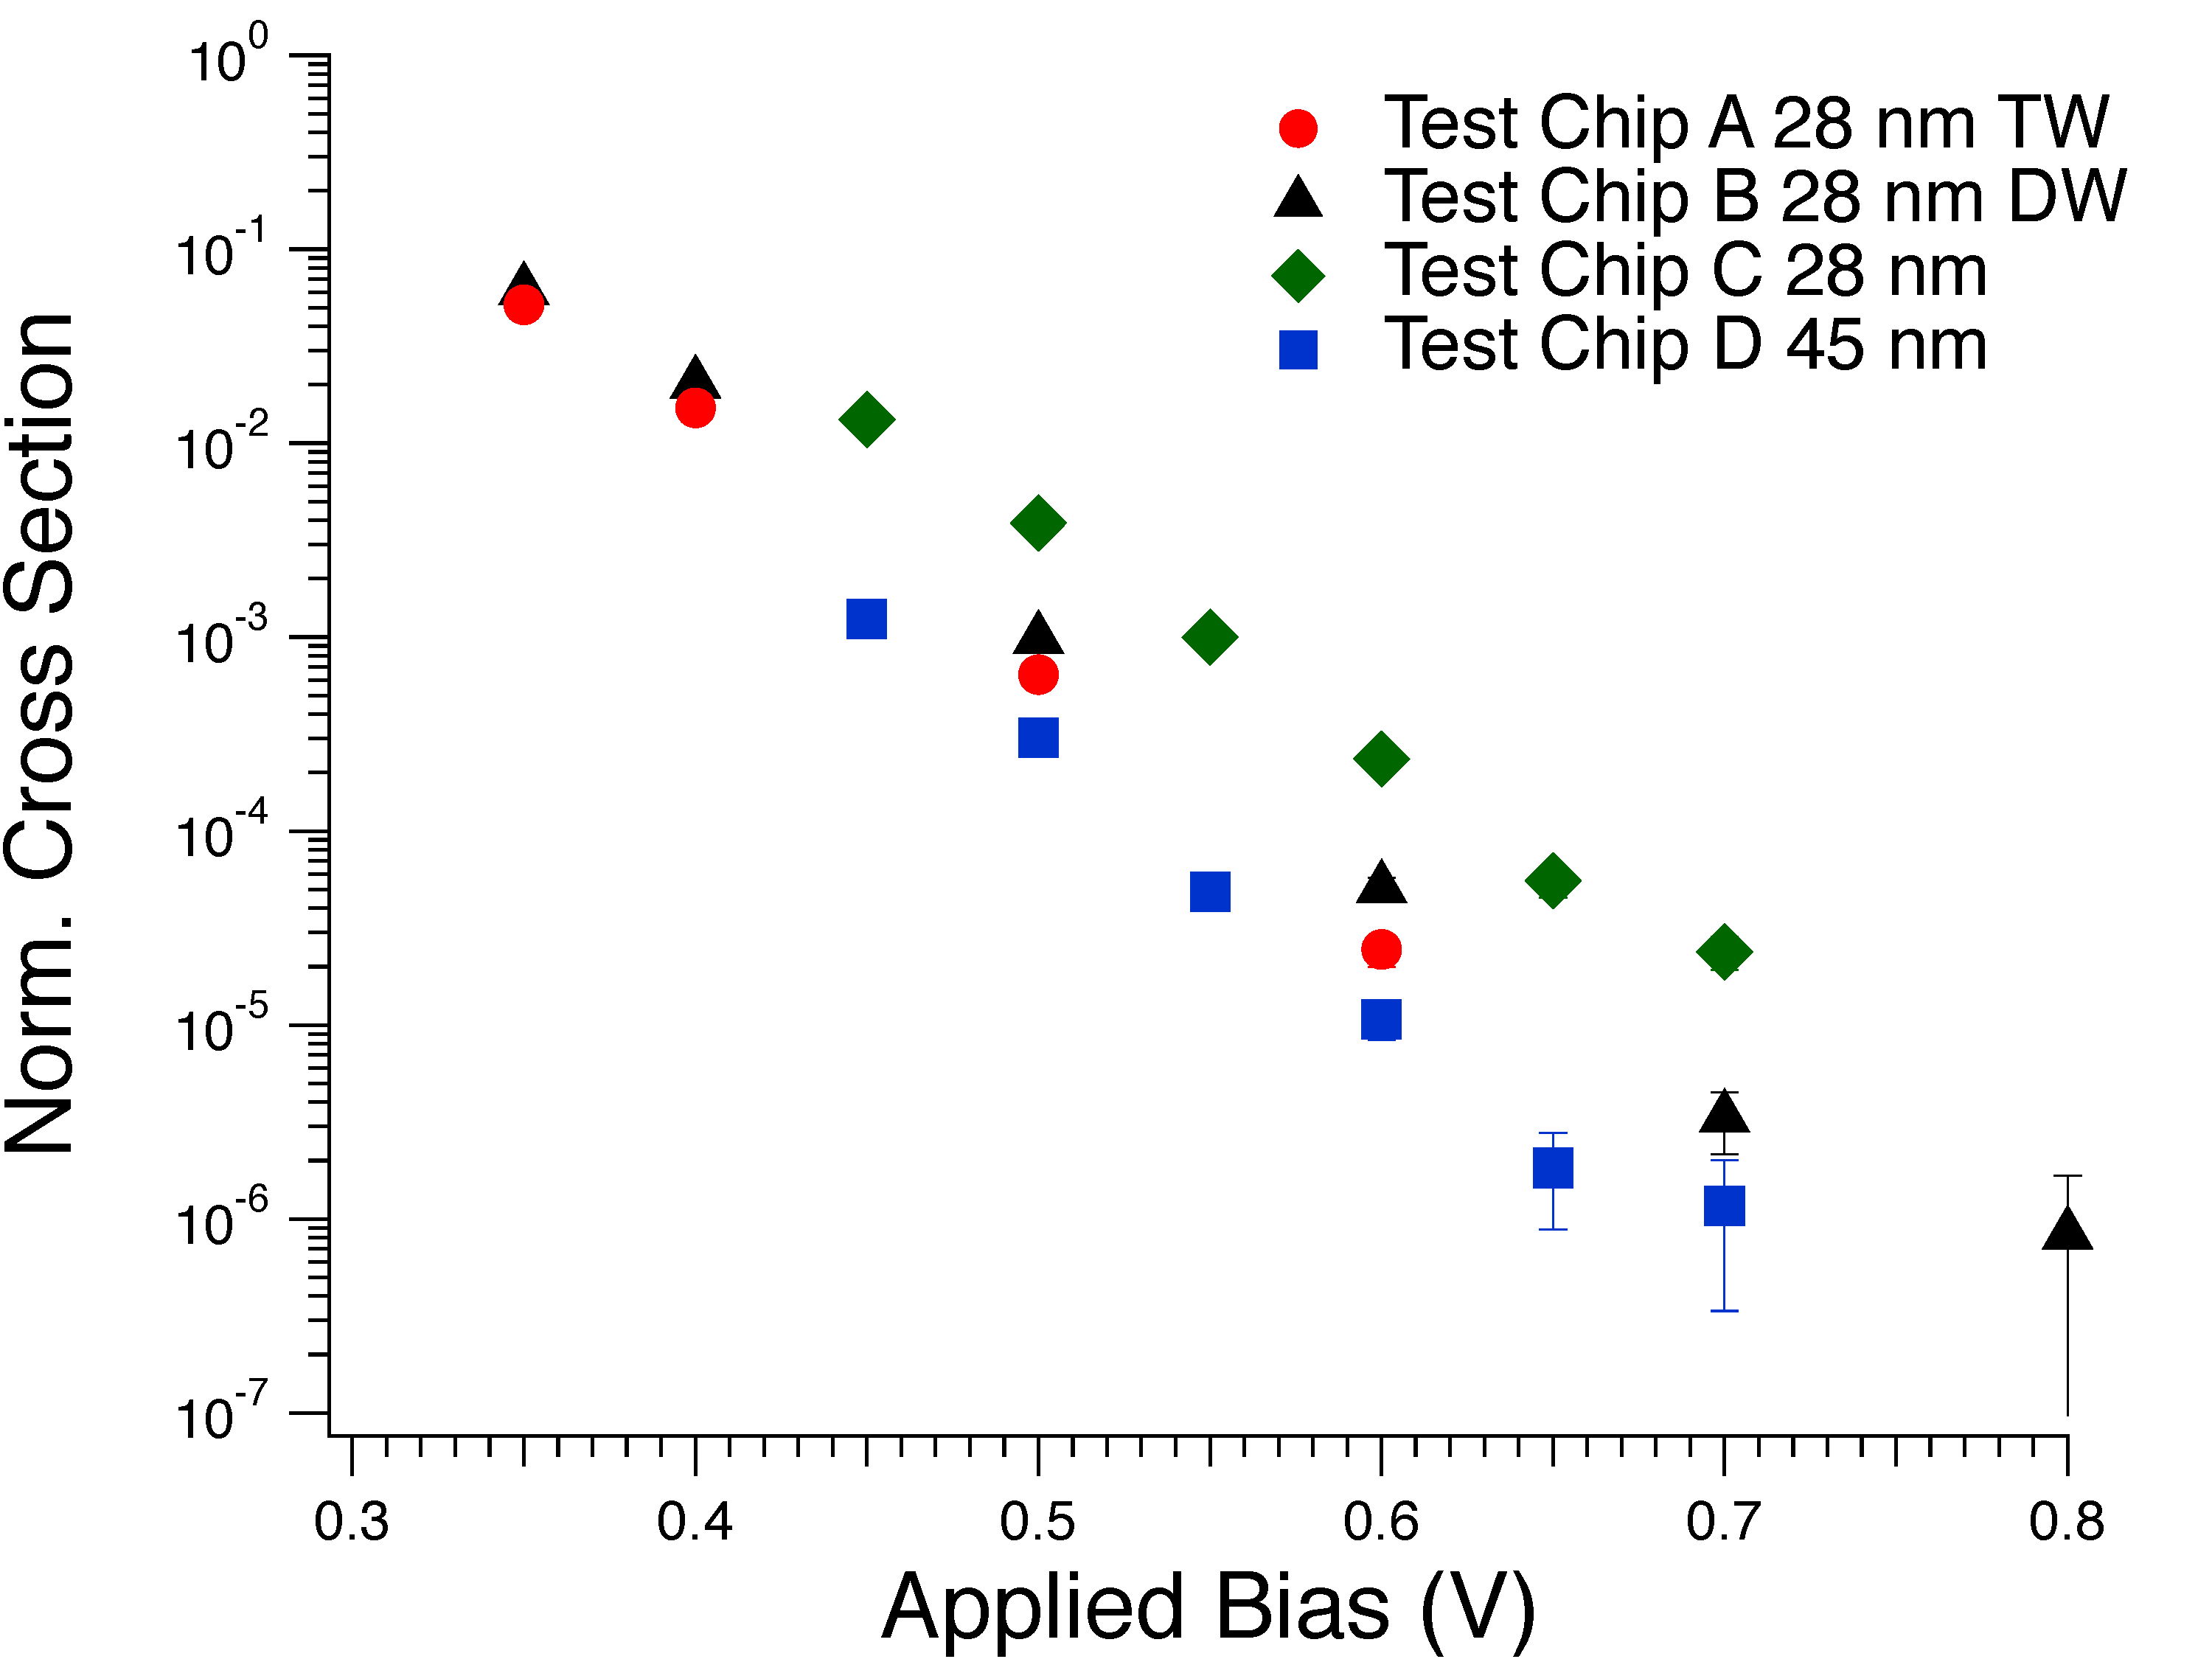
\includegraphics[width=5in]{xray_exp_sram_errors.pdf}
    \caption{Experimental errors induced during irradiation with X-rays in an ARACOR 4100 X-ray irradiator. The bias sensitivity of critical charge in SRAMs provides strong evidence of energetic electron-induced upsets in modern SRAMs.}
    \label{fig:xray_exp_seus}
\end{figure}
Fig.~\ref{fig:xray_exp_seus} plots the normalized cross-section, as described in Eq.~\ref{eq:norm_cs}, as a function of supply voltage for SRAM test chips exposed to X-rays.
Fig.~\ref{fig:xray_exp_seus} shows that errors are observed when these devices are biased between 0.35~V and 0.8~V while exposed to X-rays. 
The resulting upset cross-section of all test chips exhibits an exponential dependence on applied bias because of the voltage dependence on critical charge. 
This is consistent with well established test procedures used for assessing the single-event error rates for protons and muons \cite{Rodbell:2007vl, Sierawski:2010cj}. 
In the case of Test Chip B, upsets were observed within 10\% of the nominal supply voltage of 0.9~V, which is within the designed operating voltage range for the SRAM. 
Each of the SRAM test chips exhibits a cross-section less than the total cell area at all supply voltages, resulting in normalized cross-sections less than unity.
All observed errors had unique memory addresses, strongly suggesting that errors occurred randomly within the memory array during experiments and were not caused by repeated bit-flips in ``weak'' cells.
Again it is noted that no bit-flips occurred due to reduced bias conditions during functionality and parametric tests before and after X-ray irradiation of all test chips under all bias conditions, indicating the memory operated under stable conditions during experiments.

Photocurrents produced by the overall photon flux are generated as the result of X-ray irradiation. 
The generated photocurrent produced by the collective effect of the X-ray source can be calculated as%
\begin{equation}
    \label{eq:photocurrent}
    I_{PC} = q V \dot{D}_{SiO_2} \dot{R}_{SiO_2}
\end{equation}
where $q$ is elementary charge, $V$ is the volume of an SRAM cell, $\dot{D}_{SiO_2}$ is the dose-rate in SiO$_2$, and $\dot{R}_{SiO_2}$ is the density of electron-hole pairs generated per rad(SiO$_2$). 
The generated collective photocurrent in an individual SRAM cell is calculated with Eq.~\ref{eq:photocurrent} to be approximately 1~fA. 
SPICE simulations were performed for 28~nm SRAM test chips A and B for each experimental bias condition. 
The simulation results indicate restoring currents are greater than 100 nA at the lowest experimental supply voltage, 0.35~V. 
\begin{figure}[tb]
    \begin{center}
        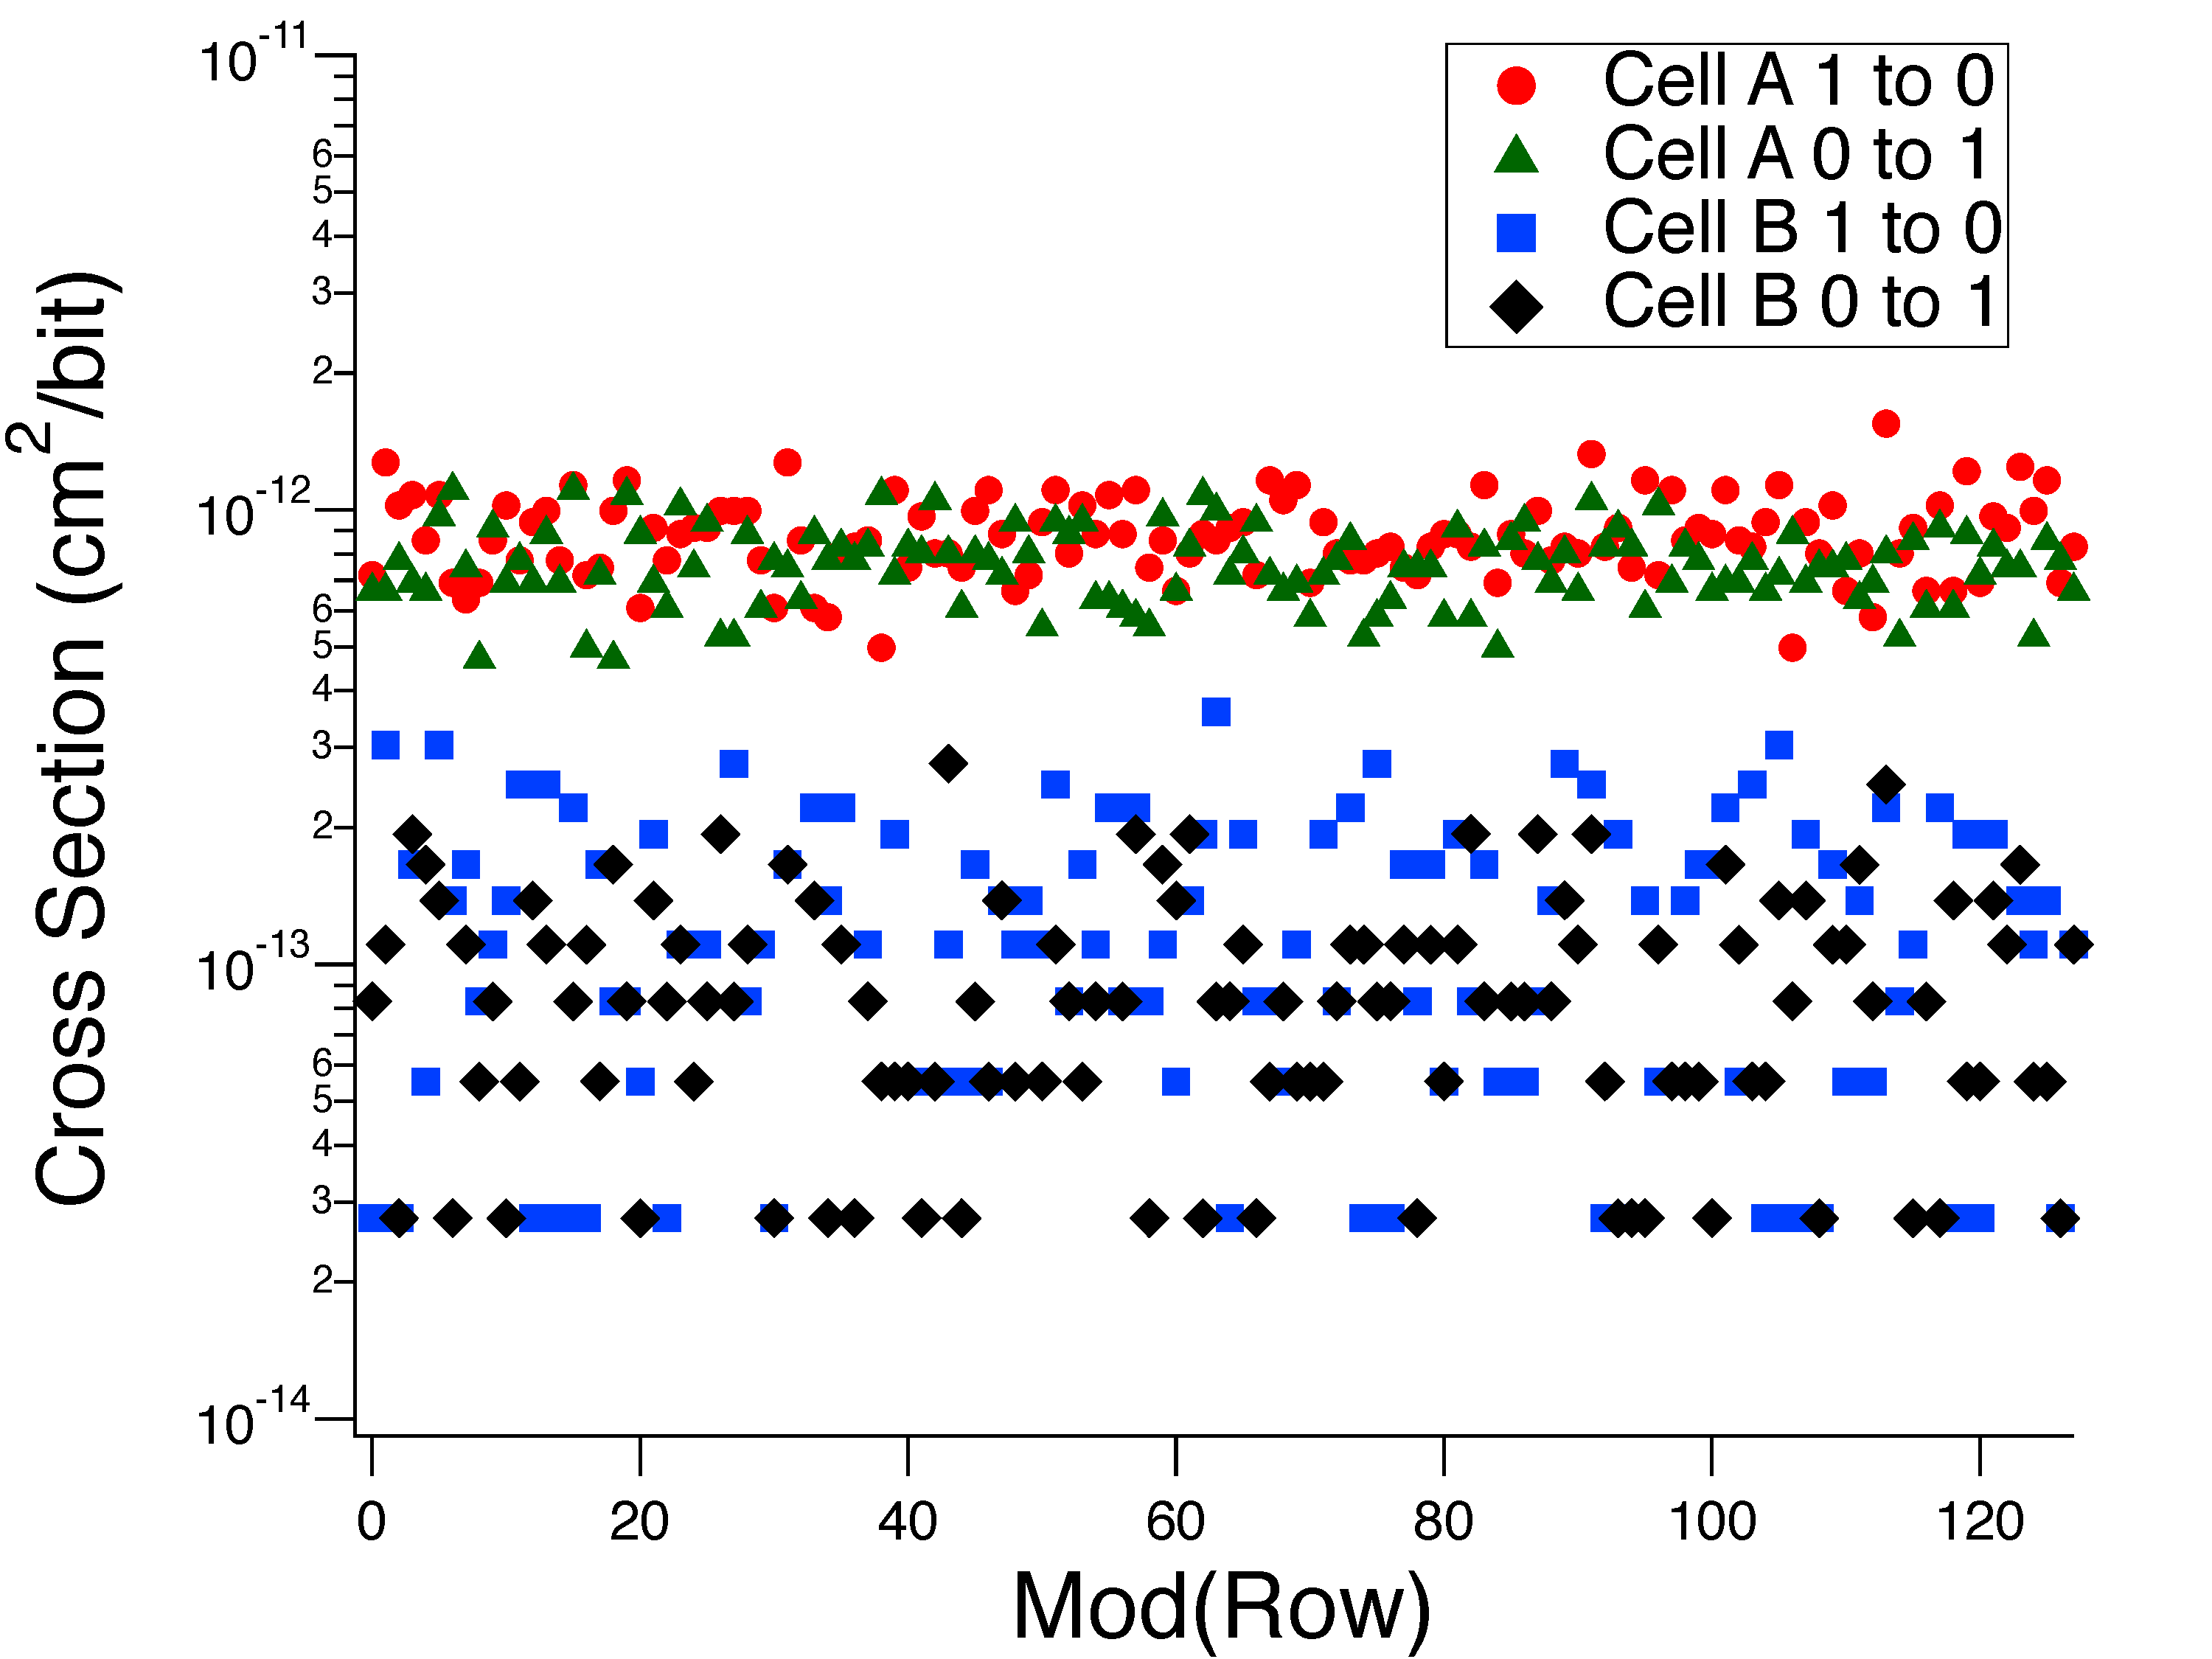
\includegraphics[width=5in]{28nm_sram_bc_cs_vs_modrow_dw_p35v.pdf}
    \end{center}
    \caption{Experimental errors induced during irradiation with X-rays in an ARACOR 4100 X-ray irradiator. Results are for Test Chip B, errors are plotted as a function of distance from row 0, corresponding to $V_{DD}$ lines, and row 128, corresponding to $V_{SS}$ lines at a supply voltage of 0.35~V. Errors occur randomly within the SRAM cell and do not preferentially occur near supply voltage or ground rails.}
    \label{fig:28nm_bc_cs_vs_modrow_dw_p35v}
\end{figure}
Fig.~\ref{fig:28nm_bc_cs_vs_modrow_dw_p35v} shows the cross-section for Test Chip B at 0.35~V as a function of distance from $V_{DD}$ and $V_{SS}$ lines.
Errors are shown to occur randomly between supply voltage and ground power metallization and do not preferentially occur near the supply voltage or ground lines, indicating that dose-rate effects do not contribute to the error rate in these experiments.
Hence, as expected, collective photocurrents generated in X-ray experiments are significantly smaller than the restoring current of SRAM cells and are incapable of causing the observed errors.

Furthermore, the probability of coincident photon events contributing to the error rate can be calculated as,
\begin{equation}
    \label{eq:prob_coincidence}
    Pr(X_1||X_2) = (\phi A_{cell} \tau)^2
\end{equation}
where $\phi$ is the incident photon flux, $A_{cell}$ is the cell area, and $\tau$ is the characteristic time for an upset event (assumed to be 10~ns). 
Evaluation of Eq.~\ref{eq:prob_coincidence} for the 28~nm and 45~nm SRAMs results in probabilities of 6.45$\times$10$^{-10}$ and 1.9$\times$10$^{-9}$, respectively, of coincident photons contributing a single upset to the experimental results. 
The contribution of coincident photons to the observed upsets on the time scale considered is therefore negligible.

Lastly, it is important to monitor the TID accumulated by the test chip, since this can lead to degradation of the memory and result in a loss of functionality \cite{Fleetwood:1987cf}. 
The dose accumulated in the experiments for the triple-well 28~nm bulk SRAM, Test Chip A, was less than 1.9~krad(SiO$_2$). 
The dual-well SRAM, Test Chip B, accumulated 5~krad(SiO$_2$) during the experiments. 
Test Chip C, a 28~nm SRAM, accumulated a dose of 5.4~krad(SiO$_2$), and Test Chip D, a 45~nm SRAM, accumulated a total dose of 11.1~krad(SiO$_2$). 
Test Chip C, a 28~nm, 32~Mbit bulk SRAM, underwent the largest change in power supply current based on measurements before and after irradiation, where the pre- and post-irradiation power supply currents were 82.7~mA and 81.5~mA, respectively.
This is a decrease in power supply current of less than 1.5\%.
Similarly, none of the other devices discussed in these experiments accumulated sufficient dose to compromise memory operation or cell integrity.

The above results and analysis demonstrate that, for the experimental conditions considered here, single energetic electrons produced by X-ray irradiation are by far the most likely cause of the observed errors within the SRAMs.
% section experimental_results (end)

\section{Comparison to Low-Energy Proton and Muon SEUs} % (fold)
\label{sec:comparison_to_low_energy_proton_and_muon_seus}
With the observation of electron-induced SEU, it is quite useful to quantify the significance of this effect relative to other well-understood phenomena. 
To this purpose, the data set presented in Fig.~\ref{fig:xray_exp_seus} is compared to SEU data sets obtained with low-energy protons and muons.

\begin{figure}[tb]
    \begin{center}
        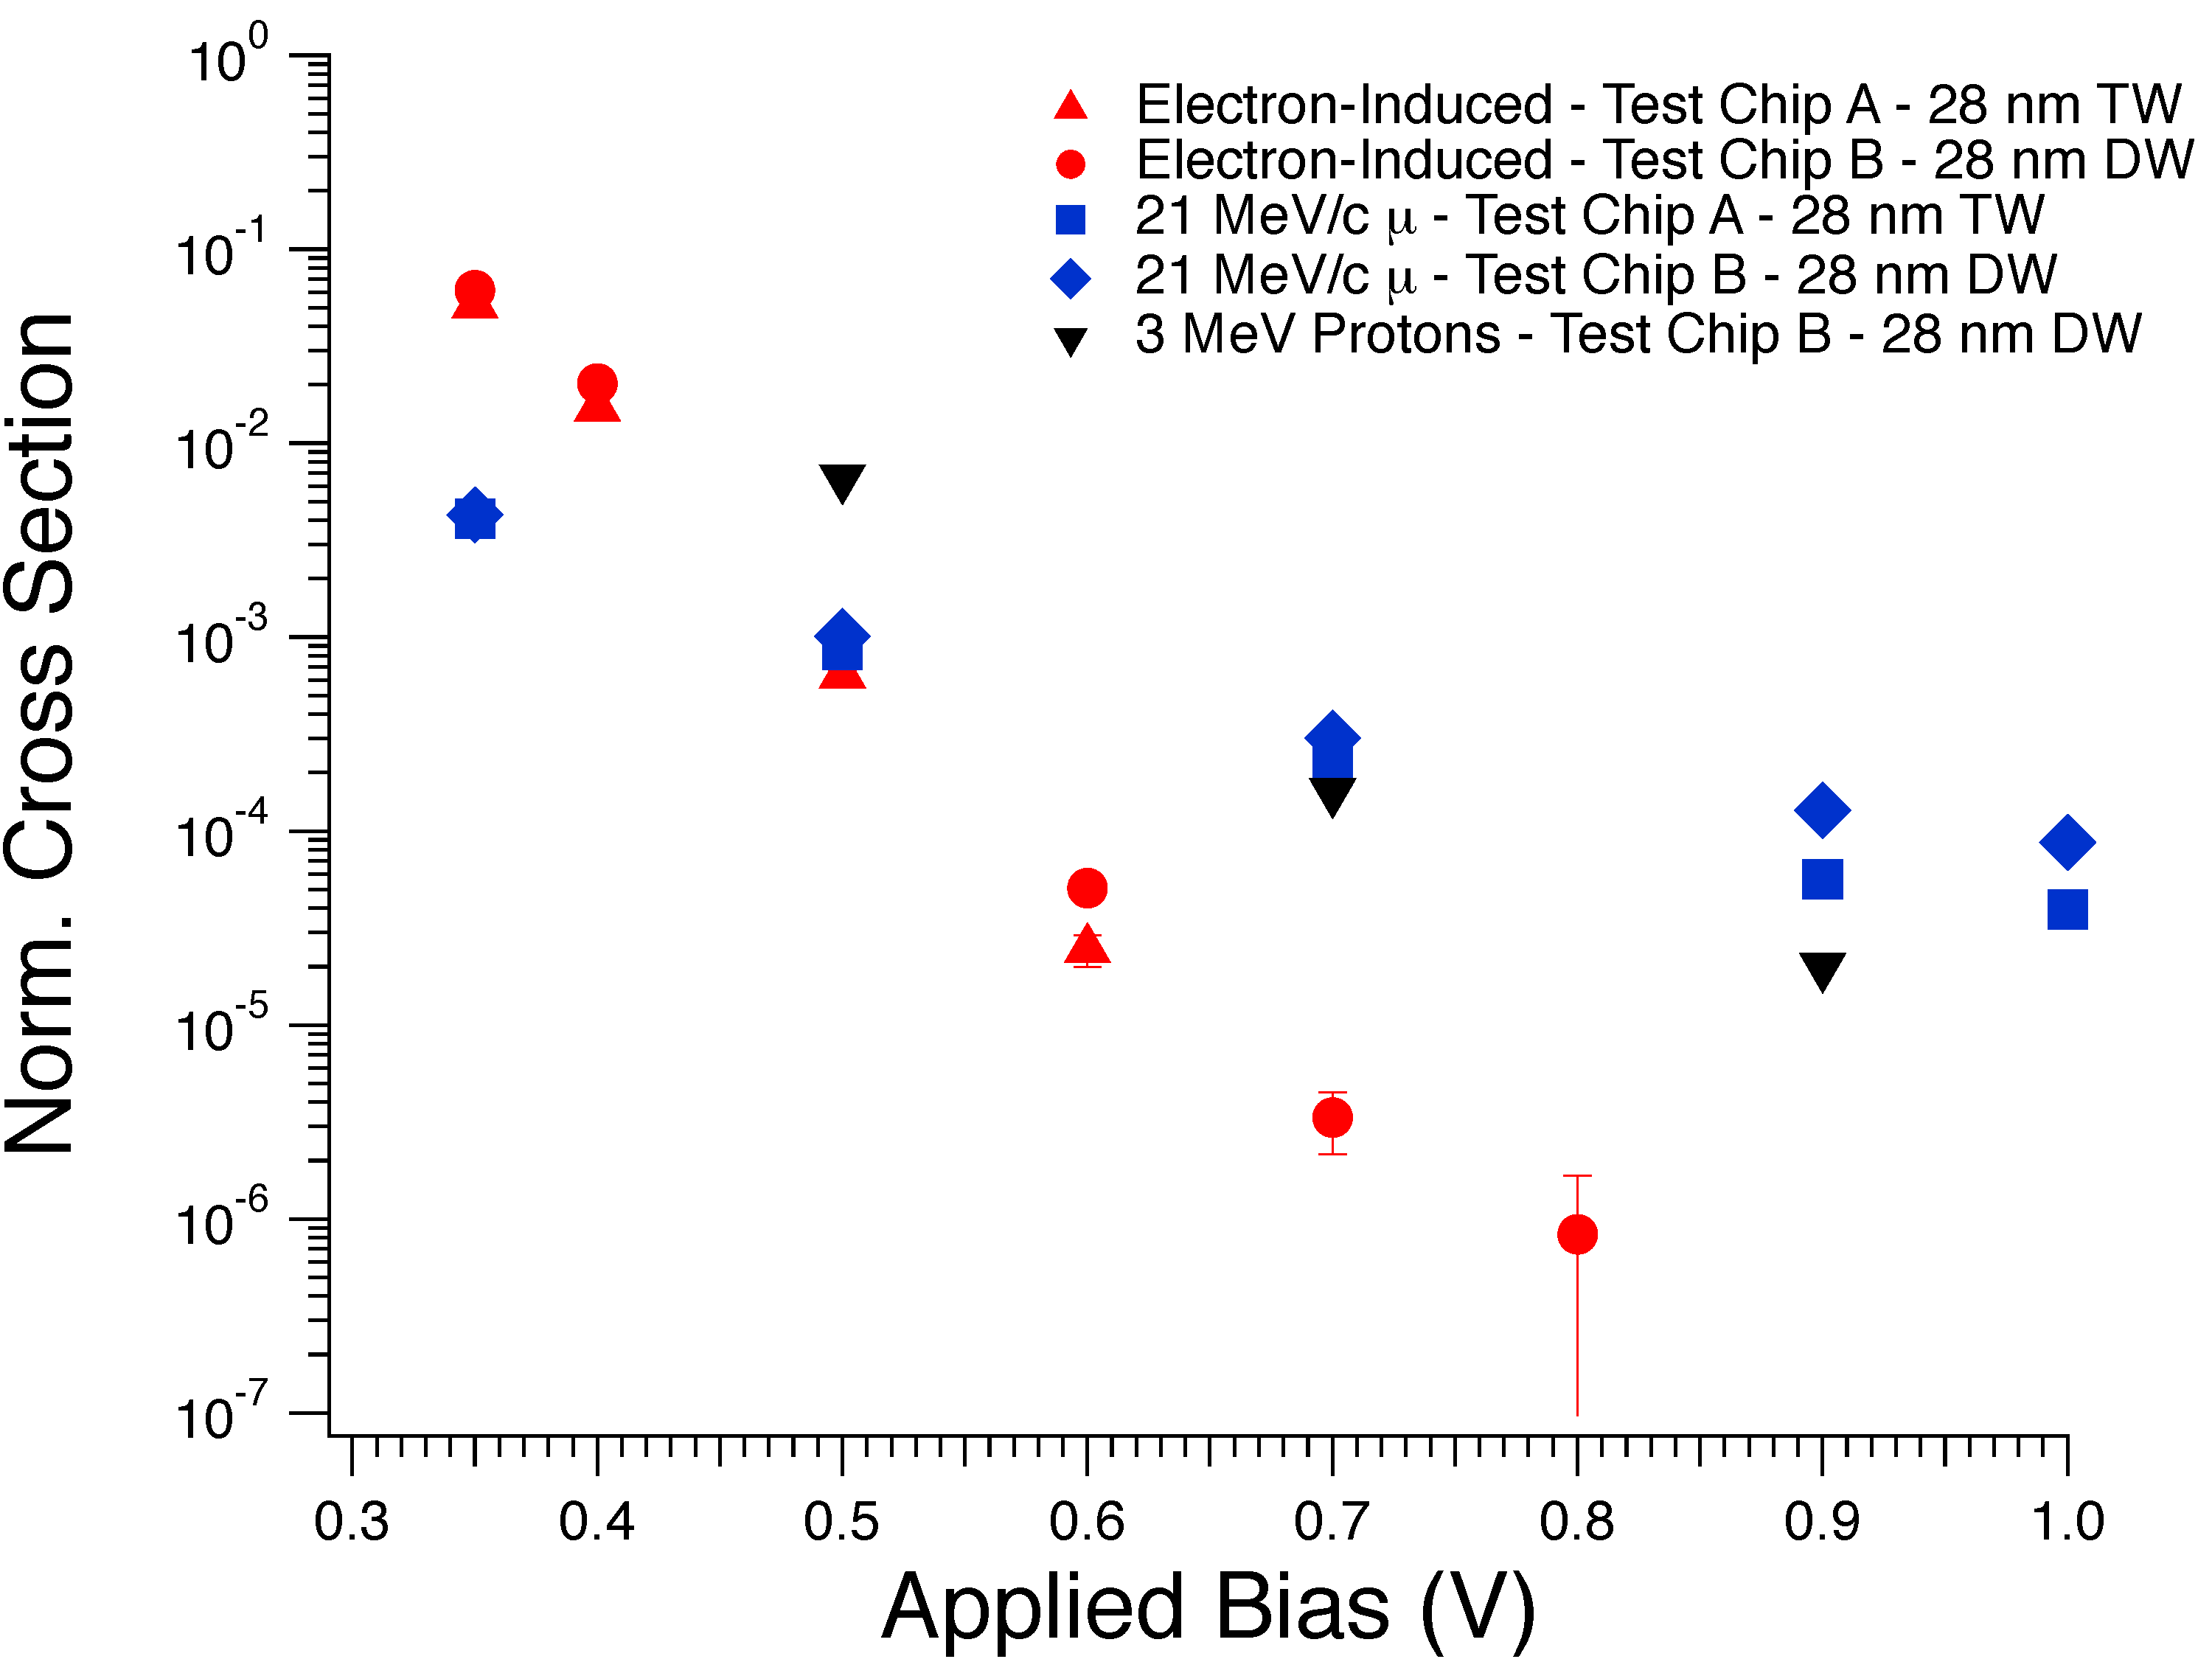
\includegraphics[width=5in]{28nm_xray_proton_muon_comp.pdf}
    \end{center}
    \caption{SEU cross-section dependence on supply voltage for electron-induced SEU cross-sections observed during X-ray irradiation, compared to low-energy protons and muons in 28~nm~(\ref{fig:28nm_xray_muon_proton}) SRAMs. Results show that under nominal bias conditions protons and muons are capable of inducing upsets in 28~nm SRAMs while this sensitivity is absent for energetic X-ray electrons generated during X-ray exposure. Under reduced bias conditions, electron-induced SEUs exhibit a larger dependence on supply voltage than muons and protons in the 28~nm technology nodes.}
    \label{fig:28nm_xray_muon_proton}
\end{figure}
\begin{figure}[tb]
    \begin{center}
        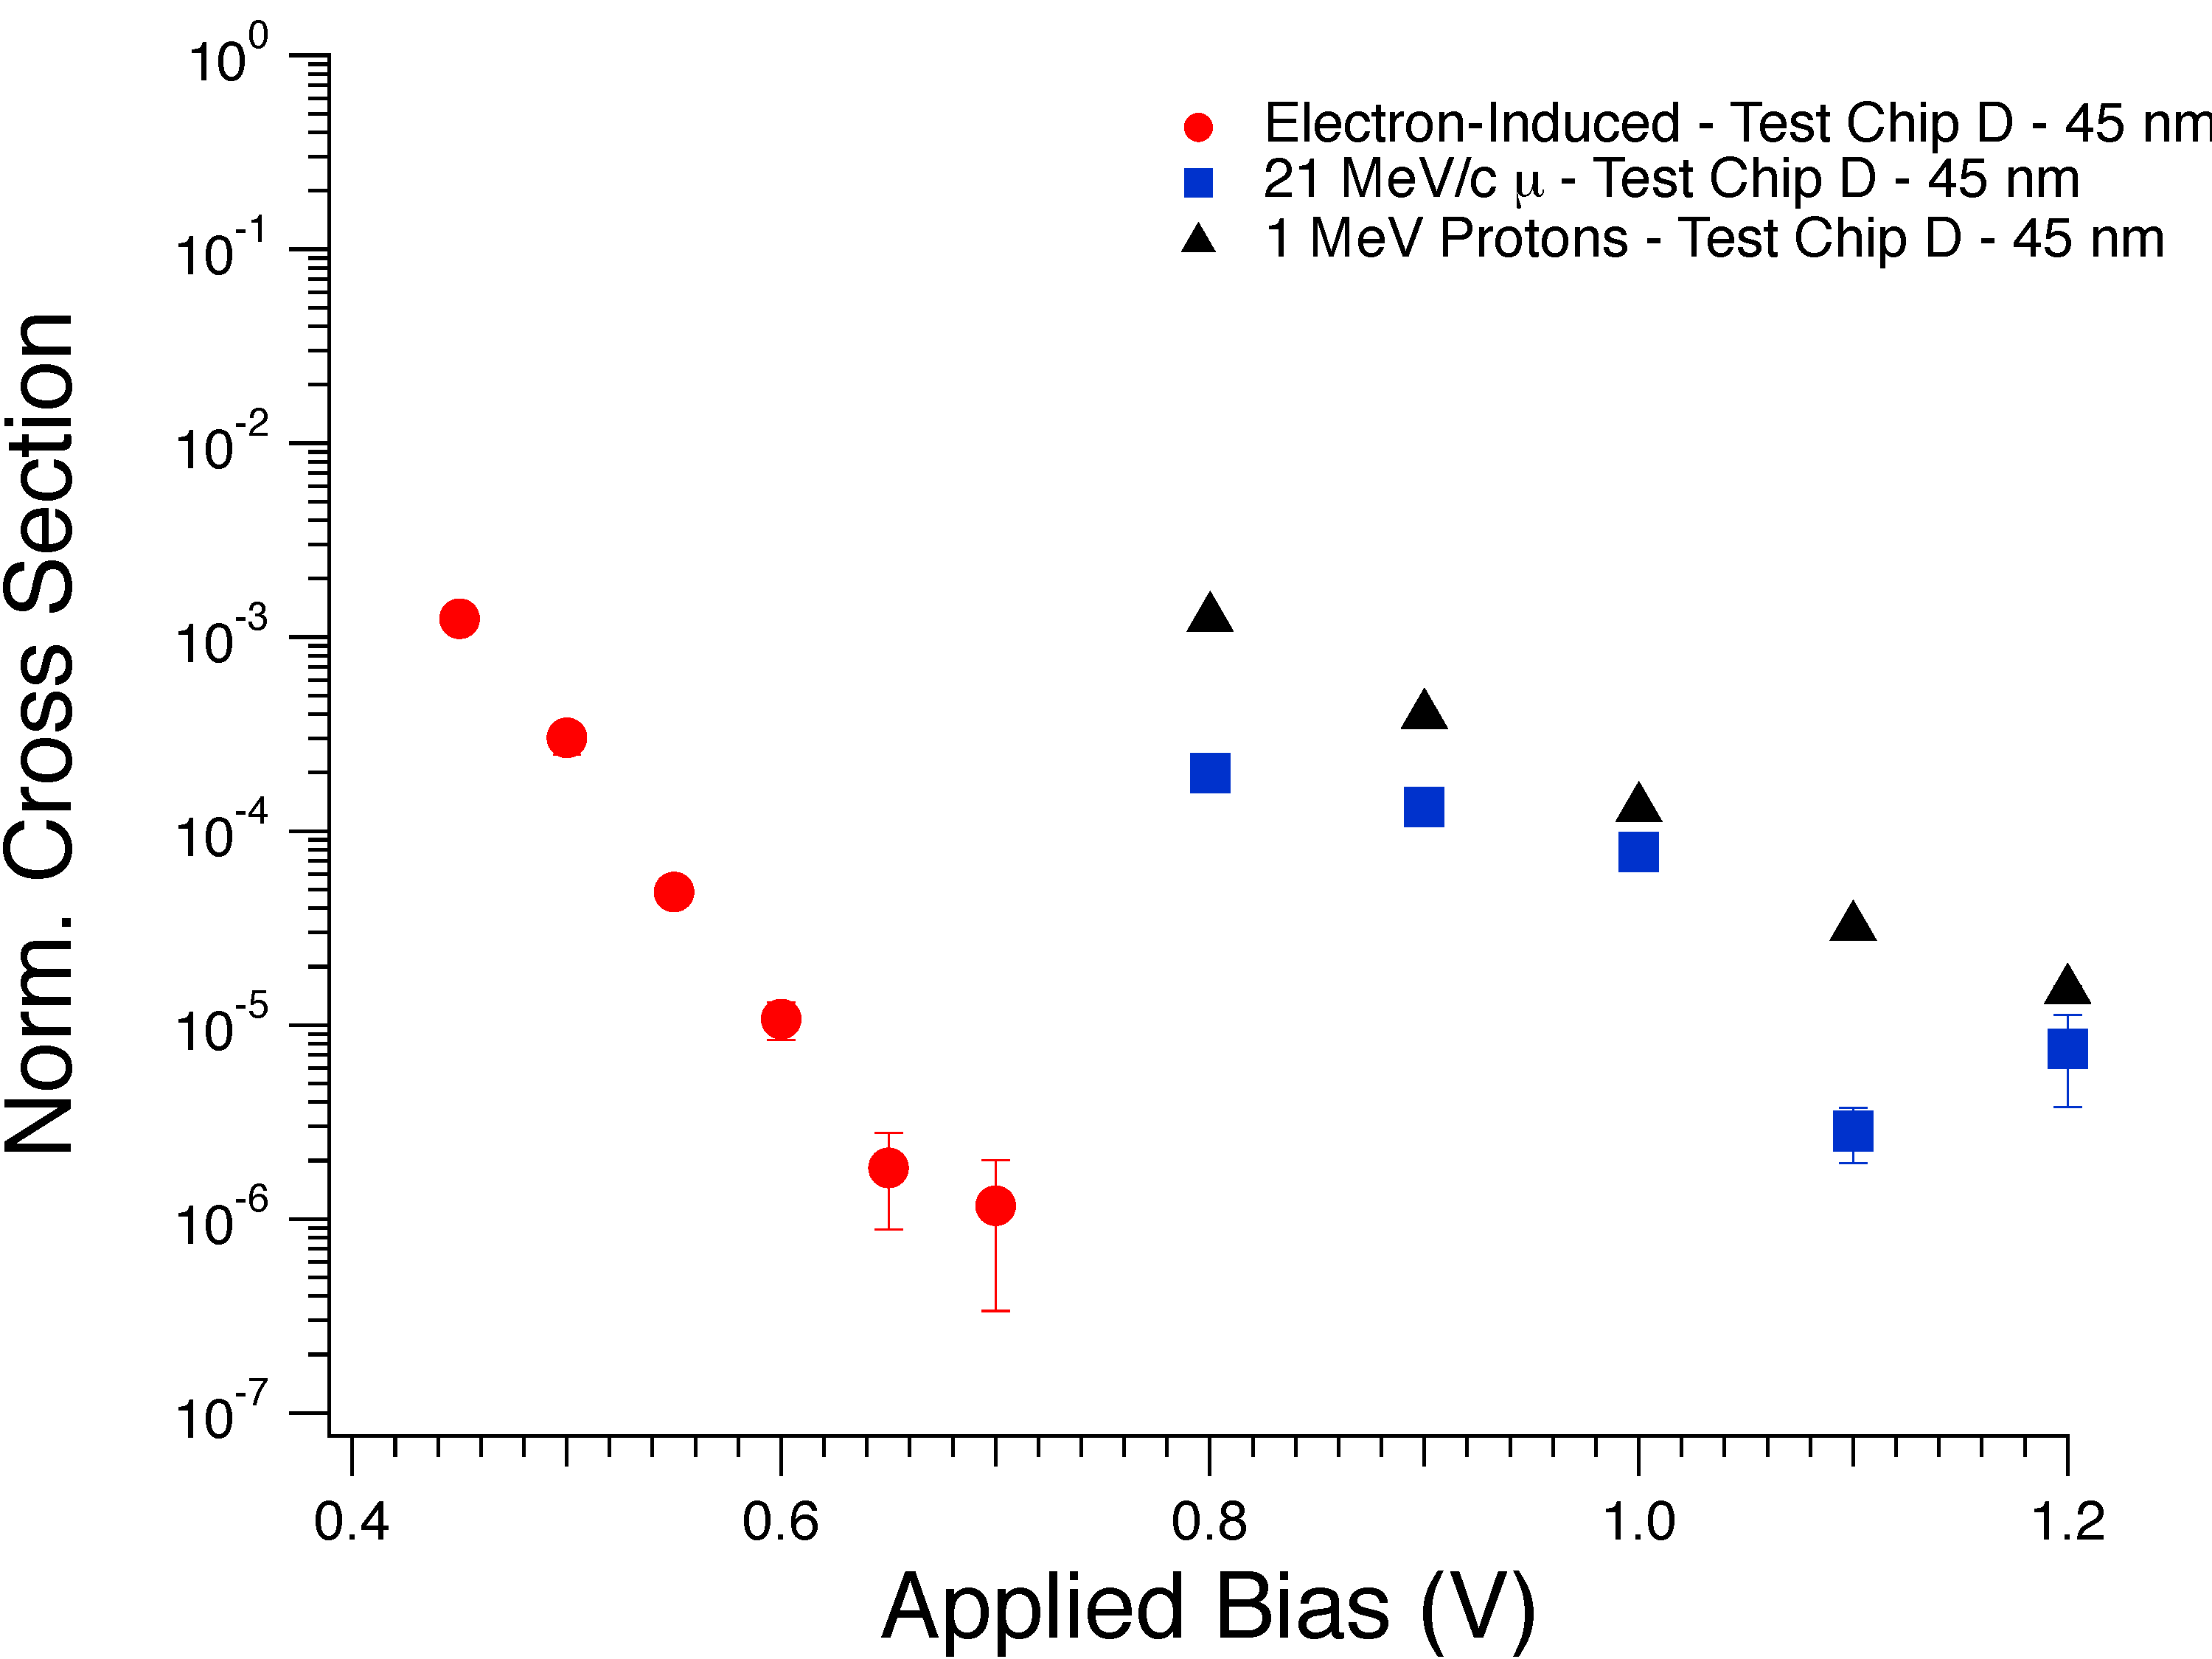
\includegraphics[width=5in]{45nm_xray_proton_muon_comp.pdf}
    \end{center}
    \caption{SEU cross-section dependence on supply voltage for electron-induced SEU cross-sections observed during X-ray irradiation, compared to low-energy protons and muons in 45~nm~(\ref{fig:45nm_xray_muon_proton}) SRAMs. Results show that under nominal bias conditions protons and muons are capable of inducing upsets in 45~nm SRAMs while this sensitivity is absent for energetic X-ray electrons generated during X-ray exposure. Under reduced bias conditions, electron-induced SEUs exhibit a larger dependence on supply voltage than muons and protons in the 45~nm technology nodes.}
    \label{fig:45nm_xray_muon_proton}
\end{figure}

Low-energy proton experiments were performed in the Pelletron facility at Vanderbilt University. 
Experiments were performed under vacuum with a monoenergetic proton beam at an energy of 3~MeV normally incident on Test Chip B and 1~MeV normally incident on Test Chip D. 
The sensitivity of the 28~nm SRAM test chip was investigated for supply voltage in the range of 0.35-1.0~V. 
The 45~nm SRAM test chip was investigated for applied biases of 0.8-1.2~V. 
The timing sequence for applied bias during experiments with low-energy protons is identical to that of Fig.~\ref{fig:exp_timing_diagram}. 
Parts were tested to a fluence of 10$^{12}$~cm$^{-2}$.

Muon experiments were performed at TRIUMF using the M15 beam line. 
Low-energy positively charged muons with a known energy distribution were normally incident on Test Chips A and B, 28~nm bulk SRAM, and Test Chip D, a 45~nm SRAM. 
The muon beam energy characterization at TRIUMF is described in \cite{Sierawski:2010cj}. 
The incident muon energy was varied by means of a tunable momentum filter \cite{Sierawski:2010cj, Sierawski:2011bn}. 
The timing sequence for applied bias during experiments with low-energy muons is identical to that of Fig.~\ref{fig:exp_timing_diagram}.
Parts were exposed to a total fluence of 6.2$\times$10$^8$~cm$^{-2}$. A normalized upset cross-section is obtained for muons and low-energy proton experiments from Eq.~\ref{eq:norm_cs}.

Figs.~\ref{fig:28nm_xray_muon_proton} and \ref{fig:45nm_xray_muon_proton} show SEU data from low-energy proton and muon experiments plotted alongside electron-induced SEU data from Fig.~\ref{fig:xray_exp_seus} for 28~nm and 45~nm test chips. 
All test chip samples exhibit exponential SEU cross-section dependence on applied bias, consistent with previous results \cite{Rodbell:2007vl, Sierawski:2010cj}. 
Electron sensitivity is observed within 10\% of nominal bias conditions for test chip B, indicating that SEUs initiated by high energy electrons may be observable in more sensitive present-generation ICs, and at nominal supply voltages for future technology nodes.
It is noted that, under nominal bias conditions, test chips A, B, and D exhibit sensitivity to muons and protons, while no events initiated by single high-energy electrons are observed. 
This indicates that high-energy electrons are much less important than protons and muons for SRAMs from these technology nodes, operating at or near nominal bias conditions.

As the applied bias is reduced, electron-induced SEUs exhibit a larger dependence on supply voltage (a larger slope) than muons and protons in the 28~nm and 45~nm technology nodes.

% section comparison_to_low_energy_proton_and_muon_seus (end)
% chapter experimental_investigation_of_electron_induced_seus (end)